%\documentclass[12pt,,a4paper]{article}%twocolumn
%\usepackage[top=2.5cm,bottom=2.0cm,left=1.5cm,right=1.5cm]{geometry} %almost-full page
\documentclass[10pt,twocolumn,a4paper]{article}%twocolumn
\usepackage[headsep=0.5cm, top=1.5cm,bottom=1.5cm,left=0.5cm,right=0.5cm]{geometry} %almost-full page

\usepackage{bm,dcolumn,amsmath,graphicx,amsfonts,amssymb,fancyhdr}


%Spacing, header sizes, title white space:
\usepackage{titling}
\setlength{\droptitle}{-2cm}
\setlength{\columnsep}{0.6cm}

%Make section headers smaller:
\usepackage[tiny]{titlesec}
\usepackage{enumitem}

%Hyperlinks:
\usepackage{hyperref}
\usepackage{xcolor}
\definecolor{cite}{rgb}{0.,0.,0.95}   % more subtle than the default blue
\hypersetup{
	colorlinks,
	linkcolor={cite},
	citecolor={cite},
	urlcolor={cite}
}


%Bibliog styles:  Emulates revtex (PRA, PRL etc.), with LINKs in bib, sorted citations,
\usepackage[sort&compress,numbers]{natbib}
\bibliographystyle{apsrev4-1}
\usepackage{doi}%<----------


\renewcommand{\bibname}{References}   %changes name to "Refs"

%% Custom functions:
\newcommand{\abs}[1]{\ensuremath{\left |#1\right |}}
\newcommand{\bra}[1]{\ensuremath{\langle #1|}}	%Dirac Bras
\newcommand{\ket}[1]{\ensuremath{|#1\rangle}}	%Dirac Kets
\newcommand{\braket}[1]{\ensuremath{\langle #1\rangle}}	%Dirac BraKets

\newcommand{\matr}[4]{\ensuremath{\begin{pmatrix}#1&#2\\#3&#4\end{pmatrix}}}	% 2x2 matrix
\newcommand{\twocomp}[2]{\ensuremath{\begin{pmatrix}#1\\#2\end{pmatrix}}}	% 2-component wavefunction

\newcommand{\threej}[6]{\ensuremath{\begin{pmatrix}#1&#2&#3\\#4&#5&#6\end{pmatrix}}}	% 3-j symbol
\newcommand{\sixj}[6]{\ensuremath{\begin{Bmatrix}#1&#2&#3\\#4&#5&#6\end{Bmatrix}}}	% 6-j symbol
\renewcommand{\v}[1]{\ensuremath{\boldsymbol{#1}}}		%bold-math for vectors
\newcommand{\vv}[1]{\ensuremath{\boldsymbol{\vec{#1}}}}		%bold-math for vectors
\newcommand{\vhat}[1]{\ensuremath{\hat{\boldsymbol{#1}}}}		%bold-math for vectors

\newcommand{\E}[1]{\ensuremath{\times10^{#1}}}	%exponent:    A x 10^y

%

\newcommand{\be}{\begin{equation}}
\newcommand{\ee}{\end{equation}}
\newcommand{\bem}{\begin{multline}}
\newcommand{\eem}{\end{multline}}



%Common symbols (use these (as opposed to doing it manually) for easy notation-changing!!
\def\d{\ensuremath{{\rm d}}}
\newcommand{\psibar}{\ensuremath{\bar\psi}}	%psi-bar
\newcommand{\psidag}{\ensuremath{\psi^\dagger}}	%psi-dagger
\newcommand{\phibar}{\ensuremath{\bar\phi}}	%psi-bar
\newcommand{\phidag}{\ensuremath{\phi^\dagger}}	%psi-dagger

\def\h{\ensuremath{\hbar}}
\def\e{\ensuremath{\epsilon}}
\def\en{\ensuremath{\varepsilon}}
\def\p{\ensuremath{\partial}}

%greek symbol short-cuts:
\renewcommand{\a}{\ensuremath{\alpha}}
\renewcommand{\b}{\ensuremath{\beta}}
\newcommand{\g}{\ensuremath{\gamma}}
\newcommand{\s}{\ensuremath{\sigma}}
\renewcommand{\t}{\ensuremath{\tau}}
\renewcommand{\k}{\ensuremath{\kappa}}
\newcommand{\vk}{\ensuremath{\varkappa}}
\newcommand{\w}{\ensuremath{\omega}}

%''mathcal''
\def\CT{\ensuremath{{\cal T}}}
\def\CL{\ensuremath{{\cal L}}}

% For nicely formatting units
\newcommand{\un}[1]{\ensuremath{\,{\rm{#1}}}} % For nicely formatting general units
\newcommand{\kms}{\ensuremath{\,{\rm km\,s}^{-1}}}
\newcommand{\ev}{\,\textrm{eV}}
\newcommand{\kev}{\,\textrm{keV}}
\newcommand{\mev}{\,\textrm{MeV}}
\newcommand{\gev}{\,\textrm{GeV}}



%%
\usepackage[normalem]{ulem}
\definecolor{newc}{rgb}{0.,0.6,0.4}
\newcommand{\new}[1]{{\color{newc}#1}}
\newcommand{\old}[1]{{\color{red}\sout{#1}}} %
\newcommand{\note}[1]{{\color{orange}{${}^*$({#1})}}}
%\renewcommand{\new}[1]{#1}
%\renewcommand{\note}[1]{#1}
%\renewcommand{\old}[1]{#1}
%

\renewcommand{\abstractname}{~\\[-1.0cm]}
\renewcommand{\contentsname}{~\\[-1.1cm]}

\setcounter{tocdepth}{1}
\usepackage[titles]{tocloft}
\setlength{\cftbeforesecskip}{1.5pt}


%\renewcommand{\today}{December 11, 2018} % XXX

%=================================================

%\title{\Large DiracSCAS: Method}
%\author{
%B.\ M.\ Roberts
%}
%\date{\today}
%\title{}


\pagestyle{fancy}
\fancyhead[L]{DiracSCAS: Method}
\fancyhead[R]{B.\ M.\ Roberts -- \today}
\begin{document}

%-------------------------------------------------------------------------------
\twocolumn[
\begin{@twocolumnfalse}
\begin{abstract}
\vspace{0.2cm}
\noindent
This is a brief description of the methods used in the code for atomic structure calculations (for single-valence systems), and has definitions for all the relevant equations.
The code is available online:\ \href{https://github.com/benroberts999/diracSCAS}{github.com/benroberts999/diracSCAS}; see the ``readme'' file for compiling/usage instructions.
Some basic documentation for the code is also available:\ \href{https://benroberts999.github.io/diracSCAS/}{benroberts999.github.io/diracSCAS/}.
This is not meant as a complete description of the physics, but references are provided to more detailed descriptions.
\end{abstract}
\vspace{0.1cm}
\end{@twocolumnfalse}
]
%%-------------------------------------------------------------------------
%\begin{abstract}
%Abstract
%\end{abstract}
%%-------------------------------------------------------------------------

%=========================================================

{\footnotesize
\tableofcontents
}

%======================================
\section{Radial Dirac equation (spherical potentials)}


Using atomic units\footnote{$\h=m_e=e=|e|=1$, $c=1/\alpha\approx137$}, the single-electron Dirac equation is
\be\label{eq:Dirac}
\left(H_D - \en\right) \phi(\v{r}) = 0,
\ee
where $H_D$ is the Dirac Hamiltonian (see, e.g., \cite{BetheBook}):
\be\label{eq:H-Dirac}
H_D = c \v{\alpha}\cdot\v{p} + c^2(\beta-1) + \hat V,
\ee
and $\v{\alpha} = \g^0\v{\g}$ and $\b=\g^0$ are Dirac matrices.
Note that we have subtracted the electron rest energy, so the total relativistic energy is $E = \en + c^2$ (for positive total energy states).
For bound states, $\phi\to0$ as $r\to\infty$ and $\phi$ is regular everywhere and thus normalisable.
The set of solutions $\{\phi_i\}$ (including the negative energy states) to (\ref{eq:Dirac}) form a complete orthogonal set/basis.
We use the standard normalisation choice, so that $\braket{\phi_i|\phi_j} = \delta_{ij}$.
%
Wavefunctions for many-electron atoms are formed from single-particle orbitals, see, e.g., Ref.~\cite{Lindgren1986}.

For spherically symmetric potentials $\hat V$, we can express the four-component single-particle orbitals in the form\footnote{We use the Dirac basis; see Appendix~\ref{sec:DiracMatrix}.}$^,$\footnote{Our notation differs from some other places: compared to Ref.~\cite{BetheBook} we have $f\leftrightarrow g$;
compared to~\cite{JohnsonBook2007} we have $f_{\rm here}= P_{\rm Johnson}$, $g_{\rm here}= -Q_{\rm Johnson}$; compared to Ref.~\cite{Dzuba1982a} we have $g_{\rm here} = \alpha g_{\rm Dzuba}$; and compared to Ref.~\cite{Sapirstein1998} we have $f_{\rm here} = g_{\rm Sapirstein}$ and $g_{\rm here}=-f_{\rm Sapirstein}$.}:
\be\label{eq:phi-orbital}
\phi_{n\k m}(\v{r}) = \frac{1}{r}\twocomp
{f_{n\k}(r)\,\Omega_{\k m}(\v{n})}
{ig_{n\k}(r)\,\Omega_{-\k ,m}(\v{n})},
\ee
where $\k = (l-j)(2j+1)$ is the Dirac quantum number, and $\Omega$ is a (two-component) spherical spinor,
\be
\Omega_{\k m} \equiv \sum_{s_z=\pm1/2} \braket{l,m-s_z ,\,1/2,s_z|j,m}\,Y_{l,m-s_z}(\v{n})\,\chi_{s_z},
\ee
with $\braket{j_1 m_1 j_2 m_2|JM}$ a Clebsch-Gordon coefficient, $Y_{lm}$ a spherical harmonic, $\v{n} = \v{r}/r$, and $\chi_{s_z}$ is a spin eigenstate [$\chi_{1/2}=(1,0)^T$, $\chi_{-1/2}=(0,1)^T$].
The terms in $\phi$ are orthonormal as: % according to: % the rules:
\begin{align}\label{eq:ffrad}
\left(n\k|n'\k\right)&\equiv\int\left(f_{n\k}f_{n'\k}+g_{n\k}g_{n'\k}\right)\d r = \delta_{n'n}\\
\braket{\k m|\k'm'}&\equiv\int\left(\Omega_{\k m}^\dag\Omega_{\k' m'}\right)\d \Omega = \delta_{\k'\k}\delta_{m'm}.
\end{align}

%$\tilde{l}=l\pm1$ for $j=l\pm{1}/{2}$

Then, we can define the radial Dirac equation in the form: % (a pair of coupled first-order ODEs):
\be\label{eq:Dirac-radial}
\left(H_r - \en\right)F_{n\k} = 0,
\ee
where we defined the {\em radial spinor},\footnote{Radial spinor defined in:~/src/Wavefunction/DiracSpinor.hpp}
\be\label{eq:F-radial}
F_{n\k} =\twocomp {f_{n\k}(r)}{g_{n\k}(r)},
\ee
and {\em radial Hamiltonian},
\be\label{eq:H-radial}
H_r = \matr 	{\hat V} 				{c(\frac{\k}{r}-\p_r )}
			{c(\frac{\k}{r} + \p_r  )}	{\hat V-2c^2}.
\ee
The 3D (spherical) Hamiltonian can also be expressed in this form by replacing $\k$ in (\ref{eq:H-radial}) with $-\hat k$ (top right) and $\hat k$ (bottom left), where $\hat k \equiv -1 - \v{\s}\cdot\v{l}$,  and $\hat k\Omega_{\k m} = \k\Omega_{\k m}$.
I will suppress the $r$ subscript and use
$\left(H - \en\right)F = 0$ and $\left(H - \en\right)\phi = 0$ interchangeably, since there is no risk of confusion.\\

%{\scriptsize \em \textbullet~Radial Hamiltonian defined in:~/src/Wavefunction/Hamiltonian.hpp}

%
%Equation (\ref{eq:Dirac-radial}) is often written in the equivalent form:
%\be
%\begin{split}\label{eq:Dirac-radial-pair}
%\left(\hat V-\en\right)f - c\left(g' - \frac{\k}{r}g\right) &= 0,\\
%\left(\hat V-2c^2-\en\right)g + c\left(f' + \frac{\k}{r}f\right) &= 0.
%\end{split}
%\ee


%------------------------------------
\subsection[Nuclear and electron potentials]{Nuclear and electron potentials\footnote{Nuclear potentials defined in:~/src/Physics/NuclearPotentials.hpp}}



For a many-electron atom, the potential term consists of the sum of the nuclear and inter-electron potentials:
\be
\hat V = V_{\rm nuc} + V_{\rm el}.
\ee
The electron potential
%\be
%V_{\rm el} = \sum_{i<j}\frac{1}{|\v{r}_i-\v{r}_j|},
%\ee
involves a large number of complicated terms and must be taken into account approximately
 (as discussed in the following sections).
For a point-like nucleus, $V_{\rm nuc} = -Z/r$;
in reality, the nuclear charge is distributed across the finite-size nucleus. %, and this must be taken into account.
%
To form $V_{\rm nuc}$, we assume the nuclear charge is distributed according to a Fermi distribution,
\begin{equation}\label{eq:FermiNuc}
\rho(r) = {\rho_0}\,{\left(1+\exp[(r-c)/a]\right)^{-1}},
\end{equation}
where $\rho_0$ is the normalisation factor,  ($\int\rho\,\d V = Z$), 
$c$ is the half-density radius, and 
$a$ is defined via the 90--10\% density fall-off {${t\equiv 4a\ln3}$} (known as the ``skin thickness''),
which we take to be $t=2.3$\,{\rm fm} for all heavy isotopes.
The half-density radius is related to $a$ and $r_{\rm rms}$, the root-mean-square charge radius, as $c = \sqrt{(5 r_{\rm rms}^2 -7\pi^2a^2)/3}$.
Then, $V_{\rm nuc}$ is obtained numerically from (\ref{eq:FermiNuc}) using Gauss' law.
The code also allows you to assume a spherical nucleus (mainly used for testing).

%The code also allows you to assume a spherical nucleus: % (mainly used for testing).
%\be
%V_{\rm nuc}^{\rm sph.}(r) = 
%-Z \left({3r_{\rm nuc}^2 - r^2}\right)/\,{2r_{\rm nuc}^3} \qquad {\rm for} \quad r<r_{\rm nuc},
%\ee
%where $r_{\rm nuc}=\sqrt{5/3}r_{\rm rms}$,
%and $V_{\rm nuc}^{\rm sph.}(r) = -Z/r$ for $r>r_{\rm nuc}$.





%======================================================
%\section{} %\label{sec:solveDirac}
\section[Numerical solution to the Dirac equation]{Numerical solution to the Dirac equation\footnote{Functions to solve Dirac equation defined in:~/src/DiracODE/}}

\subsection{Bound-state solution to local Dirac equation}\label{sec:solveDirac}

From Eq.~(\ref{eq:Dirac-radial}), we can express the radial derivative as:
\be\label{eq:dF}
\p_r F  =\frac{1}{c} \matr 	{-c\,{\k}/{r}} 	{(\en - \hat V+2c^2)}  {-(\en - \hat V)} 	 {c\,{\k}/{r}}F,
\ee
which has the familiar form of an ODE.
We solve this equation using a multi-step method.
The specific method used (Adams-Moulton method)
%\footnote{In the code, we can use the method of order 5 to 8 (default is 5; changing makes essentially no difference) -- must be set at compile time.})
 is described in detail in Ref.~\cite{JohnsonBook2007}.


In general, Eq.~(\ref{eq:dF}) will have solutions for any given $\en$. 
We are interested in the specific bound state solutions, for which $F\to0$ as $r\to\infty$, and $F(0)=0$.
To solve the bound-state problem, an initial $\en$ is guessed, and the DE is solved using the multi-step method.
Then, small adjustments are made to $\en$ until (a) we have the correct boundary conditions, and (b) we have the correct state ($n\k$) determined by the number of nodes of the orbital ($n-l-1$).
%For specific details, see Ref.~\cite{JohnsonBook2007}.


In order to use the multi-step method, a few initial points of the radial $F$ function are required.
These are determined by solving the asymptotic form of the Dirac equation analytically accounting for the boundary conditions.
It is common to expand the orbital around $r=0$ to start the procedure, and then adjust the energy until $F\to0$ at infinity.

A more numerically stable approach, however, is to solve the DE twice, once starting from $r=0$, and once from $r=\infty$~\cite{JohnsonBook2007}.
These two solutions are stepped inwards toward some central point, where the two solutions are joined -- one of the two solutions is re-scaled so that $f_0=f_\infty$ at the defined point.
Small energy adjustments are made until the lower $g$ components also match at this point (this ensures the derivatives match, and the join is smooth).
In our case, the two solutions are not joined at a single point, but are instead ``meshed'' across a few ($\simeq5$)  points around the classical turning point, defined via $V(r_{\rm ctp}) = \en$.
%(this is slightly different from Ref.~\cite{JohnsonBook2007})
The meshing procedure acts to smooth out numerical noise, and makes the method more numerically stable.
This procedure typically allows convergence of the energies to parts in $10^{16}$;
see Fig.~\ref{fig:H-SolveBS} for an example.


\begin{figure}
\centering
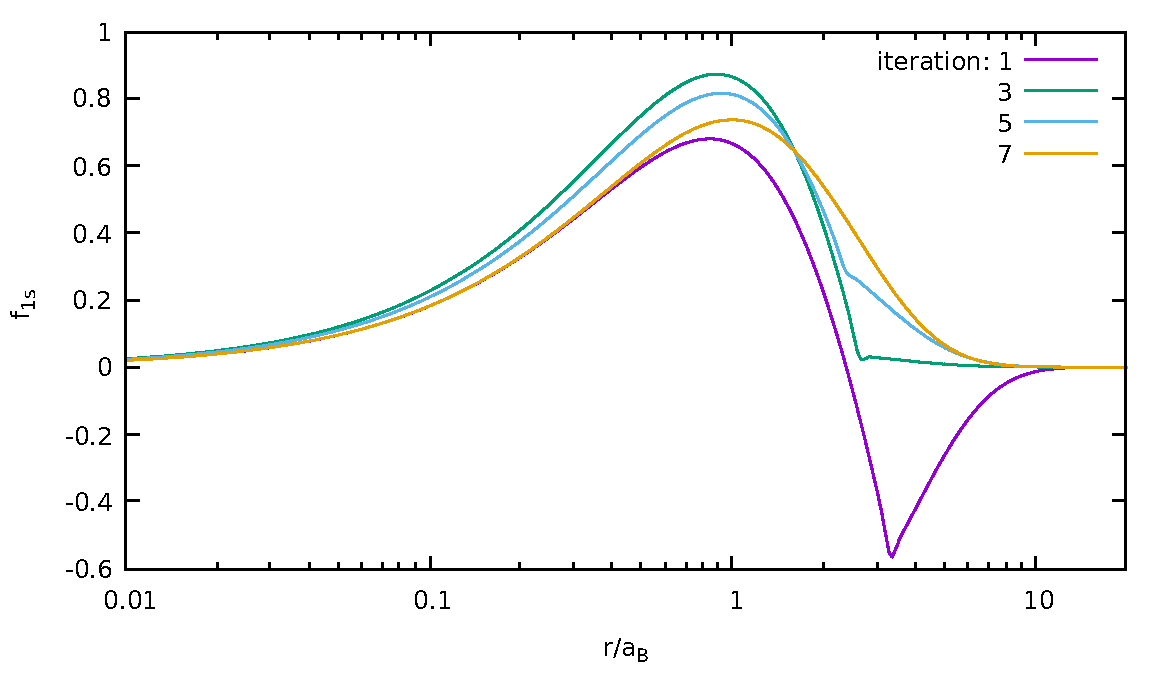
\includegraphics[width=0.4\textwidth]{img/H-SolveBS}
\caption{\small Hydrogen $1s$ orbital, as calculated at the first though 7th iteration. 
For this example, the initial energy guess was $-0.3$au, and converged to $-0.500006566..$ to parts in $10^{-16}$ in 12 iterations.\label{fig:H-SolveBS}}
\end{figure}





Note that Eq.~(\ref{eq:dF}) does not determine the normalisation for $F$, so the solutions must be normalised explicitly [Eq.~(\ref{eq:ffrad})].
Further, the sign of $F$ is also arbitrary from Eq.~(\ref{eq:dF}); we choose $f(r)$ to be positive as $r\to 0$, as is standard.


Everywhere in the code, the fine structure constant is replaced with: $\alpha\to\lambda \alpha_0$ (in atomic units, $\alpha=1/c$), where $\alpha_0\approx1/137$.
The factor $\lambda$ is a run-time input option, that is 1 by default. %It allows
For example, letting $\lambda\to0$ (i.e., $c\to\infty$) allows us to perform calculations in the non-relativistic limit.
This is a particularly useful option for checking the calculations, and for determining the sensitivity of particular observables to variations in the fine structure constant.
Modifications can also be made to the above equations to account for the finite electron/nucleus mass (reduced mass) -- but this is not implemented in the code.

%The interface to the function to that solves for the bound state is shown in Code Block~\ref{code:boundState}.
%
%\begin{code}
%\centering
%{\footnotesize
%\begin{lstlisting}
%void boundState(DiracSpinor &psi, const double en0,
%     const vector<double> &v,
%     const double alpha, int log_eps);
%\end{lstlisting}
%}
%\caption{\small\label{code:boundState}
%Function (in namespace DiracODE::) to solve local Dirac equation (\ref{eq:Dirac-radial}) for bound-state orbital psi
%(orbital must already exist - in/out parameter since this function is often called many times for same orbital as potential is updated).
%Here, en0 is the initial energy guess (energy eigenvalue is also found and stored in psi), v is the local potential
%alpha is effective $\alpha$ (=\,$\lambda\alpha_0$), and log\_eps is $\log_{10}(\epsilon)$ (i.e., put 16 to try to converge to parts in $10^{16}$).
%}
%\end{code}





%======================================================
\subsection[Radial grid]{Radial grid\label{sec:grid}\footnote{Radial grid defined in:~/src/Maths/Grid.hpp}}

The equations are solved numerically on a finite radial grid (the orbitals are stored in arrays on this grid).
We define a grid on the region from $r_0$ to $r_{\rm max}$, that has $N$ points.

We don't use a uniformly spaced grid, since the wavefunctions vary very rapidly at small distances, but rather slowly at large distances.
We define a non-uniformly-spaced radial grid ($r_i$) in terms of a uniformly spaced $u$ grid ($u_{i+1}=u_i+\delta u$).
In this case, integrals become:
\be
\int_{0}^{\infty} f(r)\,\d r \to 
\int_{r_0}^{\rm r_{max}} f(r)\,\d r \to 
\int_{u_0}^{u_{\rm max}} f(r(u))\frac{\d r}{\d u}\,\d u,
\ee
which numerically becomes:
\be
\int_{u_0}^{u_{\rm max}} f(r(u))\frac{\d r}{\d u}\,\d u \to
\sum_{i=0}^{N-1} f(r_i)\frac{\d r}{\d u}\Big|_i\,\delta u
\ee
(in the code we actually use a quadrature integration formula for the integrals).
The initial/final grid points and the grid spacings must be chosen such that the above numerical approximations are sufficiently accurate.

In the code, we can set either a logarithmic grid, defined:
\begin{align}
u &= \ln(r), \qquad
\frac{\d r}{\d u} = r,
\end{align}
or a mixed log-linear grid, defined: 
\begin{align}
u &= r + b \ln(r), \qquad
\frac{\d r}{\d u} = \frac{r}{r + b},
\end{align}
which is approximately logarithmic at small distances ($r<b$), and approximately linear at large distances (typically $b\simeq4$\,au); see Fig.~\ref{Fig:grids}.
The logarithmic grid works very well, and allows good convergence without requiring a large number of points, but works less well for highly excited states, and works quite poorly for continuum states with high energy.
The log-linear grid works well in a wide range of cases, but often needs more grid points to achieve the same numerically accuracy\footnote{The code also allows the use of linear grid -- but this requires a very large number of points to work, so should only be used for testing.}.



\begin{figure}
\centering
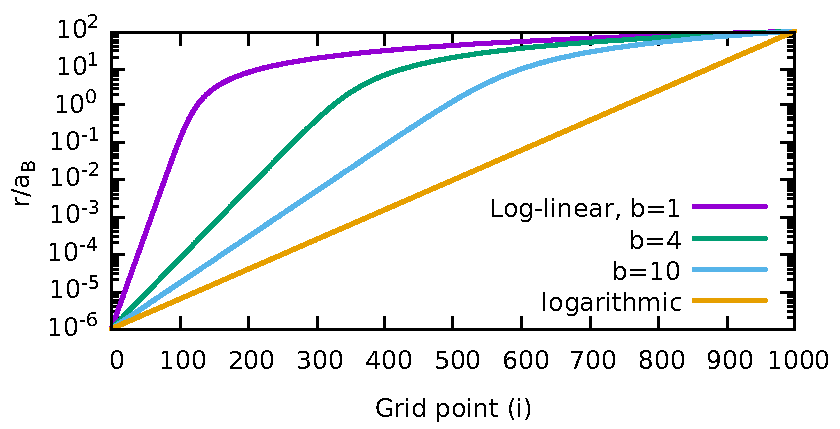
\includegraphics[width=0.43\textwidth]{img/Grids}
\caption{\small Radial distance $r_i$ as function of grid-point, $i$.\label{Fig:grids}}
\end{figure}



%======================================================
\subsection{Dirac equation involving inhomogeneous or non-local terms (Green's Method)}


This is a brief overview only; for explanations/proofs see, e.g., Ref.~\cite{Arfken2013}.
Consider the inhomogeneous Dirac equation, with extra `source' term $S$:
\be\label{eq:Green-inhomog}
\left( H_{\rm l}- \en\right)F = S,
\ee
where $H_{\rm l}$ is a Dirac Hamiltonian involving only local potential terms.
We solve this for a normalisable $F$ using the Green's method for ODEs.
First, take the homogeneous equation:
\be\label{eq:Green-homog}
\left( H_{\rm l}- \en\right) G = 0,
\ee
which we solve (for a given energy $\en$) using the regular linear ODE multi-step methods from Sec.~\ref{sec:solveDirac}.
Note that since $F$ is a normalisable solution to (\ref{eq:Green-inhomog}) $G$ will {\em not} (in general) be a normalisable solution to (\ref{eq:Green-homog}) [i.e., $G$ is not regular at the origin/infinity].
Instead, we seek two solutions, which are each bound by one of the boundary conditions; i.e., one solution that satisfies the boundary condition at the origin, $G_0$, and a second that satisfies that at infinity, $G_\infty$.
Then, the normalisable solution to (\ref{eq:Green-inhomog}) that satisfies both boundary conditions is:
\begin{multline}\label{eq:GreensSolution}
F(r) = G_\infty(r) \int_0^r \frac{G_0(r')^T \, S(r')}{c\,w(r')}\,\d r'r'
\\
+  G_0(r) \int_r^\infty \frac{G_\infty(r')^T \, S(r')}{c\,w(r')}\,\d r'
\end{multline}
($A^T B \equiv f_A f_B + g_A g_B$)
where $c=1/\alpha$. 
The Wronskian,
\be\label{eq:Green-Wronskian}
w(r) = f_\infty(r) g_0(r) - f_0(r)g_\infty(r),
\ee
should be independent of $r$.
%[the extra $c$ factor in the denominator is pulled from the definition of the derivative (\ref{eq:dF}) and can be included in $w$].

Note that this method clearly doesn't work if $w=0$; worse, the method can be numerically unstable if $S$ and $w$ are both small (if $S$ is too small, it implies the $G_{0,\infty}$ solutions will be similar, and thus $w$ will be small).
%
%The interface to the functions that solve for $G_0$ and $G_\infty$ are shown in Code Block~\ref{code:G0Ginf};
%andfor functions that solve for $F$ in Code Block~\ref{code:SolveInhomog}.
%
%\begin{code}
%\centering
%{\footnotesize
%\begin{lstlisting}               
%void regularAtOrigin(DiracSpinor &phi,
%     const double en, const vector<double> &v,
%     const double alpha);
%
%void regularAtInfinity(DiracSpinor &phi,
%     const double en, const vector<double> &v,
%     const double alpha);
%\end{lstlisting}}
%\caption{\small\label{code:G0Ginf}
%Functions (in namespace DiracODE::) to solve local Dirac equation (\ref{eq:Dirac-radial}) for orbital psi, bound only by the boundary condition at the origin (regularAtOrigin) and infinity (regularAtInfinity).
%These are needed to form the $G_0$ and $G_\infty$ solutions, respectively, needed for the Greens method -- see Eq.~(\ref{eq:GreensSolution}).
%Input parameters same as \ref{code:boundState} - but equation is just solved for given energy.
%}
%\end{code}
%
%\begin{code}
%\centering
%{\footnotesize
%\begin{lstlisting}               
%DiracSpinor solve_inhomog(const int kappa,
%     const double en, const vector<double> &v,
%     const double alpha, const DiracSpinor &source);
%
%void solve_inhomog(DiracSpinor &phi,
%     const double en, const vector<double> &v,
%     const double alpha, const DiracSpinor &source);
%
%void solve_inhomog(DiracSpinor &phi, 
%     DiracSpinor &phi0, DiracSpinor &phiI,
%     const double en, const std::vector<double> &v,
%     const double alpha, const DiracSpinor &source);
%\end{lstlisting}}
%\caption{\small\label{code:SolveInhomog}
%Functions (in namespace DiracODE::) to solve inhomogenous Dirac equation (\ref{eq:Green-inhomog}).
%All three functions do the same thing:
%First version returns a new spinor (the $F$ solution).
%Second over-writes existing spinor.
%Third also takes in (+ over-writes) spinors phi0 and phiI ($G_0$ and $G_\infty$ solutions), which can be re-used later [see, e.g., discussion below Eq.~(\ref{eq:HF-adjust-Green})].
%Note: this function solves for $G_{0/\infty}$; they don't need to be solved separately.
%Here, `source' is $S$ (\ref{eq:Green-inhomog}).
%}
%\end{code}



%======================================================
\subsection{Continuum orbitals}

We are sometimes interested in continuum orbitals that are regular at the origin (see, e.g., Ref.~\cite{BetheBook}).
For continuum orbitals of the desired energy $\en>0$, we solve using the multi-step method described above, starting from the origin and integrating outwards.
% [using a routine essentially the same as `regularAtOrigin' (Code Block~\ref{code:G0Ginf}), but this happens ``under-the-hood''].
Note that we do not have $F_c\to0$ at large $r$, and continuum orbitals cannot be normalised as above.
For most problems, however, we do require normalised orbitals.

We choose energy normalisation~\cite{BetheBook}:
\be
\int_{\en-\delta\en}^{\en+\delta\en}\braket{\en' \k m|\en \k m}\,\d\en' = 1.
\ee
This equation cannot be used directly.
Instead, the orbitals are normalised in analogy with analytic Coulomb (H-like) continuum states.
For Coulomb potentials, at large $r$ we have:
\be\label{eq:cntm-norm}
f(r) \approx \sqrt{\frac{\alpha}{\pi \beta}}\,\sin(kr + \ldots),
\ee
with
$
\beta = \sqrt{{\en}/({\en + 2c^2})}
$
(other terms in sine function are either constant, or logarithmic in $r$).
At large $r$, the atomic potential is also Coulomb-like.
We use (\ref{eq:cntm-norm}) to normalise the orbitals by enforcing the amplitude of the sine-like orbitals at large $r$ to match the analytic H-like solutions~\cite{BetheBook}.

To do this, we have to extend the radial grid out to very large distances, often much larger than the normal grid used to solve the bound-state orbitals.
The orbital is solved out to large $r$ until the amplitude/frequency of the oscillations becomes close enough to constant, and then the amplitude is re-scaled to match (\ref{eq:cntm-norm}).
After solving, the orbital is only kept up until $r_{\rm max}$, since larger distances typically do not contribute to any required radial integrals. 
%; see Code Block~\ref{code:cntm} for function interface.


%We use an `extended' grid to do this, which is formed from the regular grid (rgrid) as:\\
%~\textbullet~~\lstinline! ExtendedGrid ext_grid(rgrid, 1.2 * r_asym);!\\
%where r\_asym is the guess for the asymptotic region, found from $\en\gg Z_{\rm ion}/r$ (actual asymptotic region must be smaller than this).
%%\[
%%2\en r_{\rm asym} = Z_{\rm ion} + \sqrt{4\lambda\en + Z_{\rm ion}^2},
%%\]
%%with $\lambda=10^7$, which works reasonably well.
%Note that we also require there to be a large enough density of grid-points at large $r$ so we can sample the oscillations with high accuracy.
%This means, particularly for high energies (where oscillations of $\phi_c$ are fast), a logarithmically-spaced radial grid is no good -- details of radial grid are elsewhere.

%\begin{code}
%\centering
%{\footnotesize
%\begin{lstlisting}               
%void solveContinuum(DiracSpinor &phi, 
%     const vector<double> &v, const Grid &ext_grid, 
%     const double r_asym0, const double alpha);
%\end{lstlisting}}
%\caption{\small\label{code:cntm}
%Functions (in namespace DiracODE::) to solve local Dirac equation for continuum states of positive energy $\en$.
%Exchange potential is not included as of yet
%(approximate exchange potential as described below can be included simply into $v$).
%}
%\end{code}


%======================================================
\section[Hartree-Fock (self-consistent field method)]{Hartree-Fock (self-consistent field method)\footnote{Method implemented in:~/src/HF/HartreeFock.hpp}}


The many-body atomic Hamiltonian may be expressed as
\be\label{eq:H-manybody}
H = \sum_i h_{\rm 0}(\v{r}_i) + \sum_{i<j}\frac{1}{|\v{r}_i-\v{r}_j|},
\ee
where 
\[h_0 = c \v{\alpha}\cdot\v{p} + c^2(\beta-1) + \hat V_{\rm nuc},\]
is the single-particle Dirac Hamiltonian including only the nuclear potential.
In order to solve the single-particle Dirac equation for an $N$ electron atom, we replace the complicated electron-electron repulsion term with an approximate potential:
\be
H \approx \sum_i h_{\rm 0}(\v{r}_i) + \sum_{i}V_{\rm avg},
\ee
where $V_{\rm avg}$ is the average potential due to the other ($N-1$) electrons.
For a given $V_{\rm avg}$, this equation yields a complete set of orthogonal single-particle orbitals; many-body wavefunctions can be expressed Slater-determinants formed from these orbitals, see, e.g., \cite{JohnsonBook2007,Lindgren1986}.
This section concerns calculating $V_{\rm avg}$.


For any general ``self-consistent field method'', we start with an initial approximation for the electronic potential (e.g., Thomas-Fermi potential, or a simple parametric potential), and use this to generate a set of orbitals for the desired subset of atomic electrons (e.g., the core).
The total electron density formed from these orbital tells us the electronic charge distribution across the atom, which we use to generate a new electronic potential (Gauss' law).
In general, this new potential will be a better approximation for the true electronic potential than the initial guess.
A new set of orbitals formed in this better potential will be a better set of orbitals, which we use to generate a better-yet potential and so on, until convergence is reached.
At the end, the potential used to form the electron orbitals should be the same as the potential that is formed from the electron orbitals, and is thus self-consistent.

\subsection{Relativistic Hartree-Fock method}

The method we use to find the self-consistent potential is the relativistic Hartree-Fock method, which includes the electron exchange interaction.
This section largely follows the detailed explanation from Ref.~\cite{JohnsonBook2007}, with a few extensions.
%
In the Hartree Fock approximation, the single-particle Dirac equation is
\be\label{eq:HF}
\left(H_{\rm HF} - \en\right) \phi(\v{r}) = 0,
\ee
with the Hartree Fock Hamiltonian,
\be\label{eq:H-HF}
H_{\rm HF}  = c \v{\alpha}\cdot\v{p} + c^2(\beta-1) + \hat V_{\rm HF}.
\ee
Here, $\hat V_{\rm HF}$ is the Hartree Fock potential.
We consider mainly atoms with a single valence electron above closed shells, and take the Hartree-Fock potential to be the potential due to the $N-1$ core electrons.
This is called the $V^{(N-1)}$ potential. % ($\hat V_{\rm HF}=\hat V_{\rm HF}^{N-1}$)


By minimising the many-body energy for the single Slater-determinant electronic wavefunction (see textbook \cite{JohnsonBook2007} for details), the Hartree-Fock potential can be derived as
\begin{multline}\label{eq:Vhf-vector}
\hat V_{\rm HF}\phi_a(\v{r}_1) = \sum_{i\neq a}^{N_c}\Bigg(
\int \frac{\phi_i^\dag(\v{r}_2)\phi_i(\v{r}_2)}{|\v{r}_{12}|}\d^3\v{r}_2\,\phi_a(\v{r}_1)\\
-\int \frac{\phi_i^\dag(\v{r}_2)\phi_a(\v{r}_2)}{|\v{r}_{12}|}\d^3\v{r}_2\,\phi_i(\v{r}_1)
\Bigg),
\end{multline}
where the sum over $i$ extends over all occupied electrons $i=\{n_i,\k_i,m_i\}$.
The Coulomb integrals are computed by expanding ${r}_{12}^{-1}$ in terms of spherical harmonics (Laplace expansion) -- see Appendix~\ref{sec:app-Coulomb}.
Integrating over angles, and summing over $m$ quantum numbers we have:
\begin{align}
\label{eq:Vhf-radial}
\hat V_{\rm HF}F_a(r)& = \left(\sum_b [j_b] x_b  \,  y^0_{bb}(r)\right)F_a(r)
\notag \\  & \qquad\quad
-\frac{1}{[j_a]}\sum_b \tilde x_b^{a}\sum_k (C^k_{ab})^2\, y^k_{ab}(r) F_b(r)  \\
\label{eq:Vhf}
&\equiv V_{\rm dir}(r)\,F_a(r) + [\hat V_{\rm ex}F_a](r),
\end{align}
where now the $b$ sum extends over all occupied {\em orbitals} (i.e., $b=\{n_b,\k_b\}$),
$y_{ab}^k$ is a symmetric Coulomb integral (sometimes called Hartree screening functions, or Hartree Y functions),
%
\be\label{eq:ykab}
y^k_{ab}(r) = \int_0^\infty \frac{r_<^k}{r_>^{k+1}}\left[f_a f_b + g_a g_b\right](r')\, \d r',
\ee
with $r_{<} = \min(r,r')$, and
$C^k_{ab}$ is the angular factor,
%
\begin{multline}\label{eq:Ckab}
C^k_{ab}\equiv\bra{\k_a}|C^k|\ket{\k_b} = (-1)^{j_a+1/2}\sqrt{[j_a][j_b]}\times\\\threej{j_a}{j_b}{k}{-1/2}{1/2}{0}\pi(l_a+l_b+k).
\end{multline}
Here, $\pi(x)=1(0)$ if $x$ is even(odd), and $[x]\equiv2x+1$. 
The $x_b$ term is the occupation fraction for shell $b$, and
$\tilde x^a_b = x_b$ when $b\neq a$, but $\tilde x^a_a = 1$
($x_b=1$ for closed shell; this is an approximate way for treating HF equations for open-shell systems\footnote{The $i$ sum in (\ref{eq:Vhf-vector}) includes a sum over all occupied $m$ states; for partially filled shells, this doesn't include all $m$ values. So, to do the sum, we assume each $m$ is filled with equal probability -- i.e., that each $m$ is partially filled. We assume non-relativistic filling (e.g., $p_{1/2}$ and $p_{3/2}$ on equal footing).}).
%Note that the $a=b$ term from $V_{\rm ex}$ can also be expressed as a local potential, and though it is stored in the $V_{\rm ex}$ matrix, can actually be thought of as part of the direct potential [it actually arises from the $(n_i,\k_i)=(n_a,\k_a)$ term from the first integral on the RHS of Eq.~(\ref{eq:Vhf-vector})].
%For example, when running for the `Hartree' method (excluding exchange), it is kept.

The Hartree-Fock method is the ideal starting point for many-body calculations, since all first-order corrections to the HF potential (i.e., corrections involving single core excitations) cancel exactly~\cite{Lindgren1986}.
Corrections to energies and wavefunctions only arise at the second-order of perturbation theory.



\subsubsection*{Hartree-Fock algorithm:}
\begin{itemize}[topsep=3px]
\setlength{\parskip}{1pt} \setlength{\itemsep}{0pt plus 1pt}
%\item Use a local approximation (guess) for $V_{\rm el}(r)$\
%to form an initial set of core orbitals
\item Form initial set of core orbital using guess for $V_{\rm el}(r)$\footnote{Essentially any approximation will do, so long as the combined nuclear and electronic potentials have $V(r\to0)\approx - Z/r$, and  $V(r\to0)\approx - \xi/r$, where $\xi=1$ for a neutral atom. I use a simple parametric potential~\cite{Green1969}.}
\item Begin HF routine:
	\begin{itemize}\setlength{\parskip}{1pt} \setlength{\itemsep}{0pt plus 1pt}
	\item Form new $V_{\rm dir}$, Eq.~(\ref{eq:Vhf-radial})
	\item For each orbital
	\begin{itemize}
	\item Form new $V_{\rm exch}\phi$, Eq.~(\ref{eq:Vhf-radial})
%	\item Guess new energy based on change in $V$
	\item Solve inhomogeneous Dirac Equation (Sec.~\ref{sec:hf-orbital})
	\item Adjust energy until $\phi$ is eigenstate (Sec.~\ref{sec:hf-adjustEn})
%	\item Damp orbitals (and/or potentials)
	\end{itemize}
%	\item Define $\epsilon_{\rm HF} = |(\en_{new} - \en_{\rm old}) / \en_{\rm new}|$
%	\item Continue HF routine until $\epsilon < \epsilon_{\rm cut}$ for all states
	\item Continue HF routine until $\Delta\en/\en<\epsilon_{\rm cut}$ for all states
	\end{itemize}
	\item HF (core) has converged. ``Freeze'' $V_{\rm dir}$ and orbitals $\{\phi_c\}$
	\item Do HF for each valence state (from ``For each orbital'')\\
\end{itemize}


In the code, we perform the HF procedure for the core twice, first using an approximate localised form of the exchange potential $V_{\rm exch}$.
% (this first run is iterated until $\epsilon\lesssim10^{-5}$).
This extra step is not necessary, and is only done to speed up the convergence (it provides more realistic orbitals as a starting point for the non-local HF equations).
The approximate potential will be shown in Sec.~\ref{sec:hf-approx}.
%
Plots of the electron density ($\rho = \sum_n|\psi_n|^2$) for Cs are shown in Fig.~\ref{fig:ElectronDensity}, as calculated in varying approximations.

The HF procedure converges to the level of $\epsilon\simeq10^{-13}$.
The resulting core orbitals are correct eigenstates (that is, the energy calculated in the HF routine is the same as $\braket{\phi|H|\phi}$) to the level of $\sim10^{-11}$; see Table~\ref{tab:HF-testEn}.
The HF orbitals are also correctly orthogonal to better than $\sim10^{-6}$; e.g., for Cs, the orthogonality for the worst core-core and valence-valence states are calculated:
$\braket{5s_{1/2}|2s_{1/2}} \simeq 2\E{-6}$ and
$\braket{7s_{1/2}|6s_{1/2}} \simeq 1\E{-7}$.




\begin{figure}
\centering
%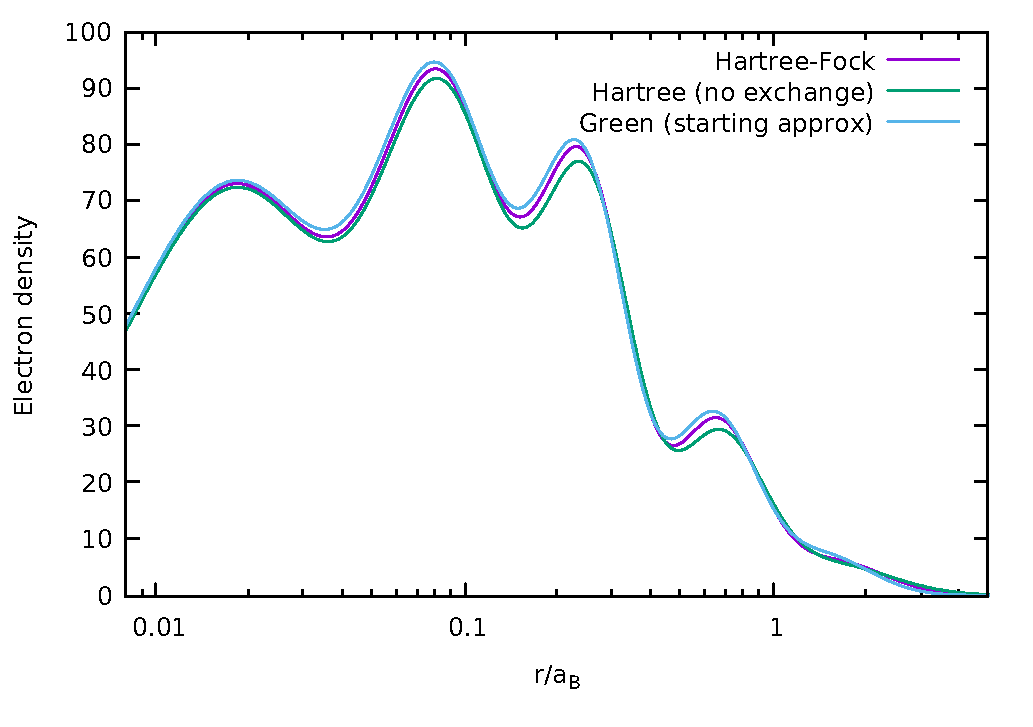
\includegraphics[width=0.44\textwidth]{img/ElectronDensityCs}
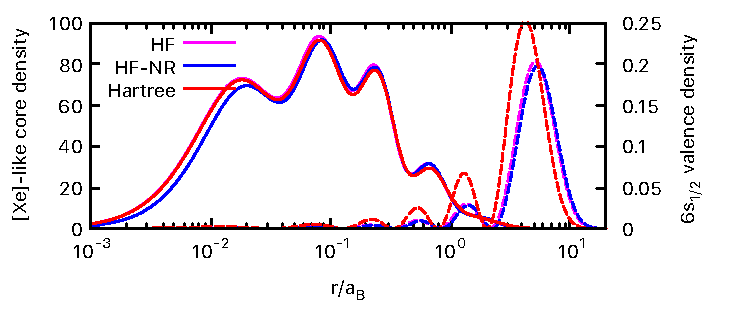
\includegraphics[width=0.5\textwidth]{img/DensityPlot-Cs}
\caption{\small Electron density $\rho = \sum_n|\psi_n|^2$ for the core (solid line) and $6s$ valence (dashed line) electrons for Cs in the relativistic Hartree-Fock (HF), non-relativistic Hartree Fock (HF-NR), and Hartree approximations. Relativistic effects ``pull'' the electrons closer to the nucleus, and the exchange interaction is crucial for valence states.\label{fig:ElectronDensity}}
\end{figure}


\begin{table*}%[h]
\small
\centering
\caption{\small Comparison of Hartree-Fock energies with expectation value of Hamiltonian for Cs (test of numerical accuracy).\label{tab:HF-testEn}}
\begin{tabular}{l D{.}{.}{5.11} D{.}{.}{5.11} r c| l D{.}{.}{3.11} D{.}{.}{3.11} r}
\hline
\hline
%Operator&lhs&rhs&$\epsilon$\\
$\psi$& \multicolumn{1}{c}{$\braket{\psi|H|\psi}$}	&  \multicolumn{1}{c}{$\en_{\rm HF}$}&  \multicolumn{1}{c}{$\epsilon^*$}	&
&
 $\psi$&  \multicolumn{1}{c}{$\braket{\psi|H|\psi}$}	&  \multicolumn{1}{c}{$\en_{\rm HF}$}&  \multicolumn{1}{c}{$\epsilon$} \\
\hline
$1s$	& -1330.11874784318	& -1330.11874784821	& -4E-12	& 	& $ 4d_{3/2}$	& -3.48561893015	& -3.48561893030	& -4E-11\\
$2s$	& -212.56445398158	& -212.56445398576	& -2E-11	& 	& $ 4d_{5/2}$	& -3.39690162346	& -3.39690162364	& -5E-11\\
$2p_{1/2}$	& -199.42945475153	& -199.42945475392	& -1E-11	& 	& $ 5s$	& -1.48980540326	& -1.48980540357	& -2E-10\\
$2p_{3/2}$	& -186.43656610582	& -186.43656610730	& -8E-12	& 	& $ 5p_{1/2}$	& -0.90789795941	& -0.90789795957	& -2E-10\\
$3s$	& -45.96974036708	& -45.96974036910	& -4E-11	& 	& $ 5p_{3/2}$	& -0.84033954719	& -0.84033954740	& -3E-10\\
\cline{6-9}
$3p_{1/2}$	& -40.44829871452	& -40.44829871568	& -3E-11	& 	& \multicolumn{4}{l}{Valence states:}\\
$3p_{3/2}$	& -37.89430454749	& -37.89430454870	& -3E-11	& 	& $ 6s$	& -0.12736806899	& -0.12736806898	& 7E-11\\
$3d_{3/2}$	& -28.30950025207	& -28.30950025207	& -1E-14	& 	& $ 7s$	& -0.05518735931	& -0.05518735931	& 4E-11\\
$3d_{5/2}$	& -27.77515677536	& -27.77515677489	& 2E-11	& 	& $ 6p_{1/2}$	& -0.08561588462	& -0.08561588462	& -5E-11\\
$4s$	& -9.51282144793	& -9.51282144936	& -1E-10	& 	& $7p_{1/2}$	& -0.04202138669	& -0.04202138668	& 2E-10\\
$4p_{1/2}$	& -7.44628469483	& -7.44628469556	& -1E-10	& 	& $ 6p_{3/2}$	& -0.08378548243	& -0.08378548242	& 1E-10\\
$4p_{3/2}$	& -6.92100118797	& -6.92100118878	& -1E-10	& 	& $ 7p_{3/2}$	& -0.04136804383	& -0.04136804383	& 5E-11\\
\hline
\hline
\end{tabular}
\\{\scriptsize$^*\epsilon \equiv (\braket{\psi|H|\psi}-\en_{\rm HF})/\en_{\rm HF}$}
\end{table*}





%-----------------------------------------------------------
\subsection{Solving the HF equation for given orbital}\label{sec:hf-orbital}

To solve the HF equation for a given orbital, we use the Green's method as outlined above.
The HF Hamiltonian is
%\be
%H = H_0 + V_{\rm nuc}+V_{\rm dir}+V_{\rm exch},
%\ee
%which we 
split in to local and non-local parts as $H_{\rm HF} = H_{\rm l}+V_{\rm nl}$, with
\begin{align}
H_{\rm l} &= H_0 + V_{\rm nuc}+fV_{\rm dir},\\
V_{\rm nl} &= (1-f)V_{\rm dir}+V_{\rm exch}.
\end{align}
Here,
\be
f=
\begin{cases}
(N_c - 1)/N_c & {\rm core} \\
 1 & {\rm valence}
\end{cases}
\ee
is chosen so that $V_{\rm l} = V_{\rm nuc} +f V_{\rm dir}\to -Z_{\rm ion}/r$ as $r\to\infty$ (otherwise, we would have $V_{\rm l}\to0$).
This is done to ensure the existence of the solution that is regular at infinity ($G_\infty$), and so that the asymptotic behaviour of the homogeneous solutions (\ref{eq:Green-homog})  match that of the final solution.

%(The procedure seems to work without doing this, but converges more slowly, and tends to be less numerically stable.
%Note that this is {\sl roughly} equivalent to including the $a=b$ term from (\ref{eq:Vhf-radial}) into $V_{\rm dir}$.)% (doing that would in some ways be ``more corect'', though once equations are solved they should be equivalent).

Then, the inhomogeneous equation has the form of Eq.~(\ref{eq:Green-inhomog}):
\be
\left( H_{\rm l}- \en\right)F = -V_{\rm nl}F.
\ee
Note that the ``source'' term in this case contains the solution $F$. 
So the equations must be solved iteratively, with some starting approximation for the source term, so that the solution at the $n$th step depends on the approximate solution from the previous step.
Further, $V_{\rm nl}$ and $H_{\rm l}$ also depend on the solution $F$ via (\ref{eq:Vhf}), and these are also formed at the $n$th step using $F^{(n-1)}$.
That is, the equation we solve at each iteration is
\begin{multline}\label{eq:inhomog-HF}
\left( H_0 + V_{\rm nuc} + fV_{\rm dir}^{(n-1)} - \en\right)F^{(n)} =
\\
 -\left( (1-f)V_{\rm dir}^{(n-1)}+V_{\rm exch}^{(n-1)} \right)F^{(n-1)}.
\end{multline}



The energy guess used for the $(n+1)$th step can be approximated as $\en^{(n)}+\delta\en$, with
\be
\delta\en \approx  \frac{\bra{F^{(n-1)}} \Delta V \ket{F^{(n)}}}{\braket{F^{(n-1)}|F^{(n)}}}
\ee
where $\Delta V = V_{\rm HF}^{(n)} - V_{\rm HF}^{(n-1)}$.
Instead of storing $F^{(n-1)}$ and $V_{\rm HF}^{(n-1)}$ for each iteration, we use $F^{(0)}$ and calculate the energy guess with respect to $\en^{(0)}$.

In general, these solutions will not be correct eigenstates of the HF Hamiltonian and won't be correctly normalised.
We therefore make small adjustments to the energy and orbital until $F$ is properly normalised and thus an eigenstate of the Hamiltonian. 
This procedure is outlined in the next subsection~\ref{sec:hf-adjustEn}.

Once the energy has been fine-tuned, and we have a normalised eigenstate, we continue the HF procedure.
To aid convergence, however, we first ``damp'' the orbitals as:
\be
F \to (1-\eta)F+ \eta F_{\rm old}.
\ee
This both increases the numerical stability, and speeds up the convergence. % (otherwise, orbitals tend to either oscillate between two values, or blow up).
Typically, $\eta\simeq0.5$; in the code, $\eta$ is initially set to a large value (0.8), and is slowly ramped down (to 0.1) over the HF iterations (0 means no damping).
So long as the equations converge, the solutions do not depend on the value chosen.



%(A slightly different method for including the non-local exchange part is given in Ref.~\cite{DzubaCPM1988pla} on pg.~462 [also \cite{DzubaCPM1989plaEn} pg.~495].)







%-----------------------------------------------------------
\subsection{Energy adjustments -- finding eigenstate}\label{sec:hf-adjustEn}




Assume the correct orbital and energy can be written as
$F +  \delta F$, and
$\en + \delta\en $,
where $F$ was the solution to Eq.~(\ref{eq:inhomog-HF}) using the trial energy $\en$.
Subbing this back into the HF Dirac equation, we find a new inhomogenous equation (to first order):
\begin{align}
(H_{\rm HF} - \en) \delta F &=  \delta\en F  \\
(H_{\rm l} - \en) \delta F &=  \delta\en F  - V_{\rm nl} \delta F,  \label{eq:HF-adjust-Green}
\end{align}
which we solve iteratively for $\delta F$ and $\delta \en$.
As the first step, we divide (\ref{eq:HF-adjust-Green}) by the unknown $\delta\en$, set $V_{\rm nl} \delta F=0$, and solve for $\tilde F\equiv\delta F/\delta\en$ using Green's method (\ref{eq:GreensSolution}).
Note that we don't need to re-solve the homogeneous equation (\ref{eq:Green-homog}), since we can re-use the $G_\infty$, $G_0$
solutions obtained when solving (\ref{eq:inhomog-HF}).

Since $(F+\delta F)$ must be normalised, we find the first guess for $\delta \en$ as (keeping only first-order terms):
\be
\delta \en = \frac{\braket{F|F} - 1}{2\braket{F|\tilde F}}.
\ee
Using  $\delta F = \delta\en\tilde F$, we form $V_{\rm nl} \delta F$ and solve (\ref{eq:HF-adjust-Green}) for $\delta F$.
Then, we make the corrections to the orbital and energy:
\be
F\to F+\delta F \, , \qquad \en\to\en + \delta\en.
\ee
This iterative procedure is continued from Eq.~(\ref{eq:HF-adjust-Green}) until the energy correction drops below a specified value
(i.e., until $F$ is properly normalised).
%The procedure converges very rapidly, and typically is converged (for $\delta\en/\en$) to parts in $10^{20}$ with just two iterations.
This procedure is very rapid; e.g., $\delta\en/\en$ typically converges to parts in $10^{20}$ with just two iterations.

Note that, so long as it was chosen appropriately, the non-local term $V_{\rm nl}$ is small, and so the $V_{\rm nl}\delta F$ term is even smaller and can be excluded entirely in this section without having much of an impact.
Including it, however, leads to better overall convergence of the HF equations.
Note that $V_{\rm nl} \delta F$ includes $V_{\rm exch} \delta F$, which must be calculated.
%; to speed things up, we restrict this calculation to include only the $k\leq1$ terms [see Eq.~(\ref{eq:Vhf})], which dominate by far.







%-----------------------------------------------------------
\subsection{Approximate ``local'' exchange potential}\label{sec:hf-approx}


There are several methods for obtaining a localised approximation to the HF potential, a common  example is the ``Hartree-Fock-Slater'' method~\cite{Slater1951}.
%
Here, I outline a slightly different method %; while decidedly more dodgy, it actually 
that gives reasonably good results.
We use this only as a starting point for the HF/TDHF procedures, so the the final result does not depend on this potential. 
The choice of a good starting approximation does, however, greatly speed up the convergence of the iterative procedures.

Introducing the notation $v^x_{ab}$ [see Eq.~(\ref{eq:Vhf-radial})], the non-local exchange part of the HF potential can be expressed
\be\label{eq:vex-vab}
 [\hat V_{\rm ex}F_a](r) = \sum_b v^x_{ab}(r) F_b(r).
\ee
It is non-local in that it cannot be expressed as $\hat V_{\rm ex}(r)\,F_a(r)$.
Multiply (\ref{eq:vex-vab}) from the right and divide  by $ F_a^\dag F_a$:
\begin{align}
 \frac{[\hat V_{\rm ex}F_a] F_a^\dag }{F_a^\dag F_a} F_a
&= \frac{\sum_b v^x_{ab}(r) F_b(r)F_a^\dag(r) }{F_a^\dag F_a} F_a(r)\\
&\approx U^{(a)}_{\rm ex}(r)F_a(r).
\end{align}
In this way we may define $U^{(a)}_{\rm ex}(r)$, which is a localised exchange potential (for state $a$).
Note that $U(r)$ is different for each state, and depends on $F_a$, and therefore must be found iteratively.

%Kind of not right wording with ``local'' vs. non-local....

In theory, this is exact except for when $F_a^\dag F_a=0$.
In practice, it is very numerically unstable whenever $F_a^\dag F_a$ is small.
However, this is not a major problem, since when $F_a$ is small, we don't care what the exchange potential is.
We proceed by introducing a cut-off, $\lambda_a$, and only calculating the exchange potential when $F_a$ is not small.
%
Therefore, we write
\be
 U^{(a)}_{\rm ex}(r) =  
v^x_{aa}(r) + \sum_{b\neq a} v^x_{ab}(r) \Lambda(r)
\ee
with
\be
\Lambda(r) = 
\begin{cases}\dfrac{F_a^\dag(r) F_b(r)}{F_a^\dag F_a} & |F_a(r)|>\lambda_a\\
0&\mathrm{otherwise}
\end{cases}
\ee
%
Of course, we don't apply the cut-off when $b=a$ in the sum, since here the cancellation is exact and there is no numerical instability.
In fact, this $a=b$ term actually gives the dominating contribution to the exchange potential. 
Partly, the reason this method gives such good results already is that the dominating case is treated exactly.

In the code, the cut-off is taken as
$
\lambda_{a} = 10^{-2} |f_a|^{\rm max},
$
where  $|f|^{\rm max}$ is the maximum magnitude for the upper $f(r)$ component of $F_a$.
Making the cut-off too small introduces numerical instabilities.
%
This potential leads to very good approximations for the HF orbitals and energies, and as such leads to very quick convergence of both HF and TDHF equations.
For example, with normal grid choices, the energies agree with complete HF energies to five digits, and the core orbitals are orthogonal to the level of $10^{-4}- 10^{-5}$.






%======================================================
\section[Finite basis of orbitals]{Finite basis of orbitals\label{sec:finite-basis}\footnote{Method implemented in:~/src/Wavefunction/BSplineBasis.hpp}}

In many problems in perturbation theory, a summation over the full (infinite) set of orbitals is required.
In theory, a basis of HF orbitals can be used for this.
However, such a basis generally converges very slowly, requires a very large radial grid, and the solutions become numerically unstable for low energies.
Further, sum over all states must include the integral over all positive- and negative-energy continuum states, which can be a significant contribution.
%
Instead, it is common to introduce a finite basis for the radial Dirac equation, see, e.g., Ref.~\cite{Johnson1988}.
%
We assert that all orbitals go to zero at the boundary of a subset of the radial grid, $r_{\rm max}$.
This is equivalent to placing the atom in the centre of an infinite spherical ``square-well'' potential.
In this case, a complete set of orbitals can be approximately expanded in terms of a finite number of states, which includes the $\en>0$ continuum states.
So long as the size of the cavity is large compared to typical radius of orbitals we are directly interested in, the results should be independent of the cavity size.




%----------------------------------------------------------------
\subsection{B-spline basis}\label{sec:Bsplines}


\begin{table*}%[h]
\small
\centering
\caption{\small Comparison between energies of spline (DKB) basis orbitals and finite-difference Hartree Fock orbitals.
The basis was constructed using 50 B-splines of order 7 in a cavity of radius 30\,$a_B$ with the first internal point at $r=10^{-5}\,a_B$ (only the first 10 splines of each symmetry are shown).
Final column shows the root-mean-square radii for the Hartree Fock orbitals. The spline basis energies agree very well (better than parts in $10^6$) with the Hartree Fock energies, so long as the cavity is large compared to the typical radius of the orbital in question; for higher orbitals, where this is not the case, the energies diverge significantly. [$\epsilon=(A-B)/A$]\label{tab:splines-energies}}
\begin{tabular}{l D{.}{.}{5.7} D{.}{.}{5.7} D{.}{}{3.3} D{.}{.}{2.2} l D{.}{.}{4.7} D{.}{.}{4.7} D{.}{}{3.3} D{.}{.}{2.2}}
\hline
\hline
 &  \multicolumn{4}{c}{$s_{1/2}$} &  &
   \multicolumn{4}{c}{$p_{1/2}$}  \\
\cline{2-5}\cline{7-10}
$n$ &  \multicolumn{1}{c}{$\en_{\rm spline}$} &  \multicolumn{1}{c}{$\en_{\rm HF}$} &\multicolumn{1}{c}{$\epsilon$}
 &\multicolumn{1}{c}{$\braket{r^2}^{1/2}_{\rm HF}$}& &\multicolumn{1}{c}{$\en_{\rm spline}$} &  \multicolumn{1}{c}{$\en_{\rm HF}$} &\multicolumn{1}{c}{$\epsilon$}
 &\multicolumn{1}{c}{$\braket{r^2}^{1/2}_{\rm HF}$}\\
\hline
1	& -1330.1186542	& -1330.1188558	& -2{\rm e}.-7	& 0.03	&& 	& 	& 	& \\
2	& -212.5644469	& -212.5644963	& -2{\rm e}.-7	& 0.12	&& -199.4294948	& -199.4295038	& -5{\rm e}.-8	& 0.10\\
3	& -45.9697097	& -45.9697486	& -8{\rm e}.-7	& 0.32	&& -40.4482937	& -40.4483086	& -4{\rm e}.-7	& 0.31\\
4	& -9.5127994	& -9.5128206	& -2{\rm e}.-6	& 0.74	&& -7.4462753	& -7.4462846	& -1{\rm e}.-6	& 0.77\\
5	& -1.4898011	& -1.4898044	& -2{\rm e}.-6	& 1.88	&& -0.9078963	& -0.9078975	& -1{\rm e}.-6	& 2.15\\
6	& -0.1273679	& -0.1273681	& -1{\rm e}.-6	& 6.52	&& -0.0856153	& -0.0856159	& -6{\rm e}.-6	& 8.65\\
7	& -0.055047	& -0.0551874	& -3{\rm e}.-3	& 14.58	&& -0.0411125	& -0.0420214	& -2{\rm e}.-2	& 18.16\\
8	& -0.0240059	& -0.0309525	& -3{\rm e}.-1	& 25.77	&& -0.0110954	& -0.0251205	& -8{\rm e}.-1	& 30.79\\
9	& 0.0147887	& -0.0198146	& 	& 40.11	&& 0.0314743	& -0.0167280	& 	& 46.56\\
10	& 0.0679063	& -0.0137713	& 	& 57.61	&& 0.0877553	& -0.0119427	& & 65.48\\
\hline
\hline
\end{tabular}
\end{table*}


The set of atomic orbitals are expanded as
\be
F_{n\k} = \sum_i^{2N} p_i S_i(r),
\ee
where $\{S_i\}$ are a set of $2N$ basis orbitals that form a complete set over a sub-domain of the radial grid $[0,r_{\rm max}]$ ($N$ is defined this way because of the duel set of positive/negative energy solutions to the Dirac equation).
The $\{p_i\}$ expansion coefficients are found by diagonalising the set of basis orbitals with respect to the Hamiltonian matrix.
In practise, this is done by solving the eigenvalue problem:
%\be
%H_{ij}p_i = \en S_{ij}p_i,
%\ee
%
\begin{align}\label{eq:Hij-splines}
\bra{S_i}\hat H_{\rm HF}\ket{S_j} p_i &= \en\,\braket{S_i|S_j} p_i\\
H_{ij}p_i &= \en S_{ij}p_i.
\end{align}
%
%with
%\begin{align}\label{eq:Hij-splines}
%H_{ij} = \bra{S_i}\hat H_{\rm HF}\ket{S_j} \, , \qquad
%S_{ij} = \braket{S_i|S_j}. 
%\end{align}
There are $2N$ solutions of eigenvalues $\en$ with corresponding eigenvectors $\vec{p}$, which correspond to the spectrum of stationary states; $N$ of these correspond to negative-energy ($\en<-mc^2$) states.
If the $S$ set is orthonormal, $B$ is just the identity, but in general it is not.
Note that $A$ and $B$ are positive-definite real matrices.
States of different $\k$ are orthogonal, so the $A$ matrix can be chosen to be block diagonal (in $\k$); i.e.\ the expansion may be performed separately for each $\kappa$. % using the same underlying basis functions.







The choice of basis must account for the boundary conditions for the stationary states.
A good choice of basis allows for convergence of many-body problems with fewer basis states.
%We use a B-spline basis, and write
%\be
%S_i = \twocomp{l_i(r)}{s_i(r)},
%\ee
%where $l$ and $s$ are formed from a set of $N$ B-splines, which are piecewise polynomials of order $k$.
The particular choice we use is called the Duel-Kinetic-Balance (DKB) B-spline basis as introduced in Ref.~\cite{Beloy2008};
\be\label{eq:DKB}
S_i^{\rm DKB}= \begin{cases}
\twocomp{b_i(r)}{\frac{\alpha}{2}\left(\p_r+\kappa/r\right)b_i(r)}  &  0\leq i<N \\
\twocomp{\frac{\alpha}{2}\left(\p_r-\kappa/r\right)b_{i-N}(r)}{b_{i-N}(r)}   & N\leq i<2N.
\end{cases}
\ee
full details, including on including boundary conditions, 
are given in that work (see also~\cite{Johnson1988,AMBiT2018}).
Note that the boundary conditions are met by discarding some of the underlying b-splines; when we talk of an expansion using $N$ splines, we refer only to the ones that are kept; the underlying spline basis consists of a slightly larger set~\cite{Beloy2008}.
Another common choice, which we refer to as the Notre-Dame (ND) basis~\cite{Johnson1988} may be formed with the lower-component of (\ref{eq:DKB}) set to zero for $i<N$, and the upper set to zero for $i\geq N$; this set requires extra conditions for the boundary conditions to be met~\cite{Johnson1988}.

Each B-spline, $b_i^{(k)}(r)$, is a polynomial of degree $k-1$, that is non-zero only in the interval $t_i\leq r<t_{i+k}$, where $\{t_i\}$ are a set of $(N+k-2)$ ``knots'' (the $S_i$ basis orbitals are non-zero also only in this region).
The first ``interior'' knot is placed at $r_0$ and the last at $r_{\rm max}$\footnote{The actual first knot is placed at 0; the end knots are repeated $k$ times.}, and the rest are distributed uniformly along the $u$ radial grid (see Sec.~\ref{sec:grid}).
%(if we are using a logarithmic grid, they will distributed exponentially along $r$, see Sec.~\ref{sec:grid}).
The piecewise nature of the splines simplifies the evaluation of integrals, and acts to make the $A$ and $S$ matrices banded, which can typically be solved with high numerical precision.
%,Quiney1987

%    The first interior knot is placed at $r_0$, and the last at $r_{\rm max}$; the basis orbitals are defined only inside this region (and are zero outside).
%    By default, this is the same as the total radial grid, but t

The basis orbitals are typically defined on a smaller sub-domain of the radial grid.
The benefit of restricting the radial sub-domain for the basis is that reasonable completeness can be achieved with fewer basis functions.
However, increasing $r_0$ too much loses the low-$r$ behaviour of the basis orbitals, and making $r_{\rm max}$ too small loses the correspondence between the ``real'' and basis orbitals.
The ideal choice of sub-domain depends on the specifics of the problem.



Table \ref{tab:splines-energies} shows the energies of spline orbitals, using 50 B-splines of order 7 in a cavity of radius 30\,$a_B$ with the first internal point at $r=10^{-5}\,a_B$.
This spline basis is orthogonal (or normal) with respect to the Hartree-Fock core to parts in $10^6$; the basis itself is orthogonal to parts in $10^{15}$.
%The basis is not orthogonal to the Hartree-Fock valence states, and is not expected to be.
Table \ref{tab:splines-hfs} shows hyperfine constants calculated using spline orbitals, which is a test of the low-$r$ performance of the orbitals.

\begin{table*}%[h]
\small
\centering
\caption{\small Magnetic dipole hyperfine constants $A$ (assuming a point-like nuclear magnetisation distribution), as calculated using the finite-difference Hartree-Fock orbitals, and the DKB basis constructed using 50 B-splines of order 7 in a cavity of radius 50\,$a_B$, with varying first internal point ($A$ is sensitive to orbitals at small radial distances). [$\epsilon=(A-B)/A$]\label{tab:splines-hfs}}
\begin{tabular}{l D{.}{.}{1.9}  D{.}{.}{1.9} D{.}{}{2.6} | D{.}{.}{1.9} D{.}{}{2.6} | D{.}{.}{1.9} D{.}{}{2.6}}
\hline
\hline
% &  \multicolumn{1}{c}{} & \multicolumn{6}{c}{$A_{\rm Spline}$, $\epsilon$}\\
 &   & 
\multicolumn{2}{c}{$r_0 = 10^{-4}\,a_B$} &
\multicolumn{2}{|c|}{$10^{-5}\,a_B$} &
\multicolumn{2}{c}{$10^{-6}\,a_B$} \\
\cline{3-8}
$n$ &  \multicolumn{1}{c}{$A_{\rm HF}$} & 
 \multicolumn{2}{c}{$A_{\rm Spline}$, $\epsilon$} & 
  \multicolumn{2}{|c|}{$A_{\rm Spline}$, $\epsilon$} & 
   \multicolumn{2}{c}{$A_{\rm Spline}$, $\epsilon$} \\
\hline
1	& 3.9180\E{7}	& 3.8361\E{7}	& -2.\E{-2}	& 3.9172\E{7}	& -2.\E{-4}	& 3.9179\E{7}	& -3.\E{-6}\\
2	& 4.6208\E{6}	& 4.5209\E{6}	& -2.\E{-2}	& 4.6199\E{6}	& -2.\E{-4}	& 4.6207\E{6}	& -3.\E{-6}\\
3	& 9.3463\E{5}	& 9.1437\E{5}	& -2.\E{-2}	& 9.3446\E{5}	& -2.\E{-4}	& 9.3462\E{5}	& -1.\E{-5}\\
4	& 1.9822\E{5}	& 1.9392\E{5}	& -2.\E{-2}	& 1.9819\E{5}	& -2.\E{-4}	& 1.9823\E{5}	& 4.\E{-5}\\
5	& 2.7987\E{4}	& 2.7380\E{4}	& -2.\E{-2}	& 2.7982\E{4}	& -2.\E{-4}	& 2.7988\E{4}	& 5.\E{-5}\\
6	& 1.4337\E{3}	& 1.4022\E{3}	& -2.\E{-2}	& 1.4334\E{3}	& -2.\E{-4}	& 1.4336\E{3}	& -4.\E{-5}\\
7	& 3.9394\E{2}	& 3.8532\E{2}	& -2.\E{-2}	& 3.9386\E{2}	& -2.\E{-4}	& 3.9394\E{2}	& -2.\E{-5}\\
8	& 1.6448\E{2}	& 1.6397\E{2}	& -3.\E{-3}	& 1.6760\E{2}	& 2.\E{-2}	& 1.6763\E{2}	& 2.\E{-2}\\
\hline
\hline
\end{tabular}
\end{table*}













%======================================================
\section[External fields + matrix elements]{External fields + matrix elements\label{sec:tdhf}\footnote{Method implemented in:~/src/HF/ExternalField.hpp}}

\subsection{Time-dependent Hartree-Fock}\label{sec:tdhf}


In the presence of a time-varying external field with frequency $\omega$, the orbitals will contain time-varying perturbations:
\be
\psi \to \psi + \delta\psi = \psi +  X e^{- i\w t}+ Y e^{ i\w t},
\ee
with $\en\to\en+\delta\en$.
Keeping terms only to first-order, the corrections are seen to satisfy the equations (e.g.,~\cite{DzubaHFS1984}):
%\begin{align}
%\left( H_{HF} - \en -\w \right)X &= -\left(\hat h + \delta V - \delta \en \right)\psi \notag\\
%\label{eq:tdhf}
%\left( H_{l} - \en -\w \right)X &= - V_{nl}X - \left(\hat h + \delta V - \delta \en \right)\psi
%\end{align}
\begin{equation}\begin{split}
\label{eq:tdhf}
\left( H_{HF} - \en -\w \right)X &= -\left(\hat h + \delta V - \delta \en \right)\psi \\
\left( H_{HF} - \en +\w \right)Y &= -\left(\hat h^\dag + \delta V^\dag - \delta \en \right)\psi ,
\end{split}\end{equation}
where $\hat h$ is the tensor operator for the external field with rank $k$.
%
Here, $\delta V$ is the correction to the HF potential arising due to the corrections $\{X^{(c)},\,Y^{(c)}\}$ to each of the core orbitals, $c$.
%This is a very important correction that will be discussed in the next section; for now, however, we will drop this term and just focus on solving these inhomogenous equations. 


The corrections are not (in general) states of definite angular momentum, but do have definite parity.
We expand $X$ and $Y$ in terms of partial waves ($\chi$ and $\eta$) of definite $\k$ ($j^\pi$):
\begin{equation}\begin{split}
\label{eq:dPsi-pw}
X^{a,m_a} &= \sum_{\a,m_\a} X_{\a,m_\a}\\
 &= \sum_{\a,m_\a}(-1)^{j_\a-m_\a}\threej{j_\a}{k}{j_a}{-m_\a}{q}{m_\a}\chi_{\a, m_\a}.
% \\
%Y^{(a,m_a)} = \sum_{\a,m_\a} (-1)^{j_\a-m_\a}\threej{j_\a}{k}{j_a}{-m_\a}{q}{m_\a}\eta_{\a, m_\a}.
\end{split}\end{equation}
The superscript refers to the unperturbed state that $X$ is a correction to (here $a\equiv n_a,\k_a$).
%Here, $\chi$ and $\eta$ are regular Dirac spinors (\ref{eq:phi-orbital}).
The sum over $\alpha$ runs over all angular momentum states with $j_\alpha = j_a - k, ..., j_a+k$ and parity $\pi_\alpha = (-1)^{l_a + \pi}$ (where $\pi$ is the parity of the operator $\hat h$).
%For a scalar operator, there is only a single term in the sum.
%$|\vk|=|\k|$ (i.e., $\Delta j = 0$), with parity determined by $\k$ and the parity of the operator
%(here $\k$ is for unperturbed state $\psi_\k$, $\vk$ is for correction $\delta\psi_\vk$).
%For a vector operator, $\Delta j = \pm1,0$ and so on.
Note that $\{\chi_\a\}$ are orthogonal (and are orthogonal to $\psi$), and form a linearly independent set of solutions to (\ref{eq:tdhf}).




%================================
\subsection[Solving the TDHF equations]{Solving the TDHF equations\label{sec:tdhf-solve}\footnote{Functions to solve TDHF equation are in:~/src/HF/MixedStates.hpp}}

The $\delta V$ term in (\ref{eq:tdhf}) is very important and will be discussed in the next section. 
Here, we will ignore how it is calculated and just focus on solving the inhomogenous equations. 


%To find the solutions to (\ref{eq:tdhf}), 
As before, we express the Hamiltonian as $H =H_{\rm l} + V_{\rm nl} $: %, with
\begin{align}
H_{\rm l}&= H_0 + V_{\rm nuc} +  V_{\rm dir} +  U_{\rm x} \\
V_{\rm nl} &= V_{\rm exch} - U_{\rm x},
\end{align}
where $U_{\rm x}$ is a local approximation to the exchange potential.
In the simplest case it is $(f-1)V_{\rm dir}$, but better approximations aid the convergence (we use that from Sec.~\ref{sec:hf-approx}).
It is desirable to make  $V_{\rm nl}$ as small as possible.
%
%The $\delta V$ term is very important and will be discussed in the next section; for now, we ignore this term and just focus on solving the inhomogenous equations. 

We solve the equations iteratively, such that at the $n$th step:
\begin{multline}\label{eq:tdhf-its}
\left( H_{\rm l} - \en \pm\w \right)X^{(n)} =
 \\
 - (V_{\rm nl} X)^{(n-1)} - \left(\hat h  + \delta V- \delta \en^{(n-1)} \right)\psi_a,
\end{multline}
with $V_{nl}X= 0$ initially.
The solution for each $\a$ is
%\be\label{eq:del-phi-tdhf}
%\delta\psi_\vk = \frac{\phi_\vk^\infty}{cw}\int_0^r\left\{\phi^0_\vk|S\right\}\,r^2\d r'
%+ \frac{\phi_\vk^0}{cw}\int_r^\infty\left\{\phi^\infty_\vk|S\right\}\,r^2\d r'.
%\ee
\be\label{eq:del-phi-tdhf}
X_\a = \frac{\phi_\a^\infty}{cw}\int_0^r\left\{\phi^0_\a|S\right\}\,r^2\d r'
+ \frac{\phi_\a^0}{cw}\int_r^\infty\left\{\phi^\infty_\a|S\right\}\,r^2\d r',
\ee
where the ``source'' term $S$ is the rhs of Eq.~(\ref{eq:tdhf-its}).
(Note: the $\delta\en$ term only contributes for the $X$ term with $\a=a$.)
The $\phi_\vk^{0,\infty}$ functions here are the solutions with Dirac quantum number $\a$ to the homogenous equation (\ref{eq:Green-homog}), including both the angular part and the $1/r$.
We defined here the ``partial'' matrix elements, that include only the integral over angular coordinates:
\be
\left\{\psi_a|\hat h|\psi_b\right\} \equiv \int \psidag_a \hat h\psi_b \,\d\Omega.
\ee




We similarly define the partial reduced matrix element:
\begin{align}\label{eq:partial-rme}
\left\{\psi_a|T^k_q|\psi_b\right\} &\equiv (-1)^{j_a-m_a}\threej{j_a}{k}{j_b}{-m_a}{q}{m_b}\left\{\psi_a||T^k||\psi_b\right\}.
\end{align}
Then, in terms of the partial waves ($\chi$), the solution becomes:
\be\label{eq:del-phi-tdhf2}
\chi_\a = \frac{\phi_\a^\infty}{cw}\int_0^r\left\{\phi^0_\a||S\right\}\,r^2\d r'
+ \frac{\phi_\a^0}{cw}\int_r^\infty\left\{\phi^\infty_\a||S\right\}\,r^2\d r'.
\ee
This is done so that we only need to calculate the ($m$-independent) {\rm reduced} matrix element of $\hat h$.
The radial integral $|\chi_\a|^2$ is used to control convergence (for including the exchange term).
Using $U_x$ from Sec.~\ref{sec:hf-approx}, convergence (for a given orbital) to parts in $10^9$ is typically reached in $\sim$\,10 iterations.
% with no damping.

%What about $\delta V\psi_\k$ --- has $\vk$ ????
%No..? means we have to include all $\vk$ from sum?
%.. but only one contributes for each??

%We divide Eq.~(\ref{eq:del-phi-tdhf}) by $\Upsilon$, and solve the DE in terms of the projection
%\be
%\widetilde {\delta\psi}_\vk  = \frac{1}{\Upsilon_{\vk,\k}} {\delta\psi}_\vk.
%\ee




From perturbation theory, the correction (excluding $\delta V$ and considering the case with $\delta \en=0$) can also be expressed as:
\be
\ket{X} = \sum_n \frac{\ket{n}\bra{n}\hat h\ket{\psi}}{\en-\en_n+\omega},
\ee
which can be used to test the method.
Consider, e.g., %the matrix element:
\begin{align}
%\label{eq:tdhf-test1}
%\braket{m|X} &= \frac{\bra{m}\hat h\ket{\psi}}{\en-\en_m + \omega},\\
\label{eq:tdhf-test}
\braket{m|\chi} &= \frac{\bra{m}|\hat h|\ket{\psi}}{\en-\en_m + \omega},
\end{align}
which can be calculated both ways (lhs vs rhs); see Table~\ref{tab:tdhf-test}.
%\note{w should be different from resonance term???}


\begin{table}%[h]
\small
\centering
\caption{\small Testing TDHF method using Eq.~(\ref{eq:tdhf-test}) for Cs, with $m=6p_{1/2}$, $\psi=6s_{1/2}$ (Hartree-Fock level, no $\delta V$).\label{tab:tdhf-test}}
\begin{tabular}{llll}
\hline
\hline
Operator&(\ref{eq:tdhf-test})~lhs&(\ref{eq:tdhf-test})~rhs&$\epsilon^*$\\
\hline
$h_{\rm E1}~~~(\omega=\omega_{\rm HF})$&63.2029312&63.2025676&6\E{-6}\\
$h_{\rm E1}~~~(\omega=0)$&126.405501&126.405135&3\E{-6}\\
$h_{\rm PNC}~(\omega=0)$&-1.0700928&-1.0700932&4\E{-7}\\
\hline
\hline
\end{tabular}
\\{\scriptsize$^*\epsilon \equiv (lhs-rhs)/lhs$}
\end{table}

An important application of this technique is that it allows calculations to be done without requiring a summation over the complete set of intermediate states (replaced by solving the inhomogeneous differential equation).
This method of performing exact summation over intermediate states is sometimes called the Solving Equations, Mixed States, or Dalgarno-Lewis method~\cite{Dalgarno1955}, depending on context.
In this example (\ref{eq:tdhf-test}) the intermediate-states summation is trivial, since it involves only single operator and hence only a single intermediate state contributes. 
In general, all intermediate states (including continuum and positive energy states) contribute, so this method allows calculations without the need for a large basis.

%See also Sec.~\ref{sec:Bsplines} below for a test of the  Dalgarno-Lewis method for calculating PNC amplitudes.


Another way to test the method is to consider the parity non-conservation (PNC) amplitude, which is a correction to the (otherwise forbidden) $E1$ transition between states of the same parity, due to the parity-violating weak interaction between the electrons and nucleus (see, e.g., Ref.~\cite{GingesRev2004}).
This can be expressed as a sum over all intermediate states $n$:
\be
E_{{\rm PNC}}^{(z)} = \sum_n\frac{\bra{B}\v{d}_z\ket{n}\bra{n}h_{\rm W}\ket{A}}{\en_{A}-\en_n} + \frac{\bra{B}h_{\rm W}\ket{n}\bra{n}\v{d}_z\ket{A}}{\en_{B}-\en_n},
\label{eq:pnc-se-ss}
\ee
where $\v{d}$ is the $E1$ operator, and $h_{\rm W}$ is the PNC operator.
Using the TDHF (Dalgarno-Lewis) method as described in Sec.~\ref{sec:tdhf}, this can also be expressed in two other formally equivalent ways:
\begin{align}
E_{{\rm PNC}}^{(z)} &= \bra{B}\v{d}_z\ket{\delta A^{(W)}} + \bra{\delta B^{(W)}}\v{d}_z\ket{A} \label{eq:pnc-se-dw}\\
&= \bra{\delta B^{(d)}}h_{\rm W}\ket{A} +  \bra{B}h_{\rm W}\ket{\delta A^{(d)}}\label{eq:pnc-se-dd},
\end{align}
%(which we refer to here as the $\delta W$ and $\delta d$ method, respectively),
where $\delta A^{(W/d)}$ is the correction to orbital $A$ due to the weak/E1 interaction.
%
Comparing the results of Eqs.~(\ref{eq:pnc-se-dw}) and (\ref{eq:pnc-se-dd}) tests the numerical accuracy of the Dalgarno Lewis (solving-equations) method, and comparing these to the result of (\ref{eq:pnc-se-ss}) gives a good test of the basis.
The two forms of the Dalgarno Lewis method agree to parts in $10^8$.
Comparison between the PNC amplitude as calculated using this and the direct-summation method is in Table~\ref{tab:pnc-basis}.



\begin{table}%[h]
\small
\centering
\caption{\small 
Comparison of PNC amplitudes (at the HF level) for $^{133}$Cs as calculated using the Dalgarno-Lewis (DL) method, and direct summation using a spline basis [formed in a cavity of $(10^{-6},50)\,a_B$ using $N$ splines  of order $k$].\label{tab:pnc-basis}}
\begin{tabular}{lllll}
\hline
\hline 
&&\multicolumn{3}{c}{Direct Summation: $N/k$}\\
\cline{3-5}
Transition&DL&50/5&60/6&70/7\\
\hline
$6s-7s$&-0.73954&-0.73948&-0.73953&-0.73954\\
$6s-5d_{3/2}$&-2.4000&-2.3998&-2.4000&-2.4000\\
\hline
\hline
\end{tabular}
\end{table}



%======================================================
%======================================================




%======================================================
%\subsection{Core polarisation (RPA)}
\subsection[Core polarisation (RPA)]{Core polarisation (RPA)\footnote{Method implemented in:~/src/HF/ExternalField.hpp}}

This section largely follows Ref.~\cite{DzubaHFS1984} (see also \cite{Dzuba2018a,Manakov1986,Johnson1980,Johnson1989}).
In the presence of an external field, the core electrons become perturbed and a correction to the HF potential is induced, which leads to important corrections to the matrix elements of the external field operator.
This effect is often called core polarisation, and is particularly important since it involves corrections with single excitations from the HF core (in the absence of an external field, the lowest-order corrections to the HF potential involve two excitations).
The method described here is often referred to as the random phase approximation (RPA).


To account for core polarisation, the set of TDHF equations (\ref{eq:tdhf}) are solved self-consistently for each of the core orbitals using the method from Sec.~\ref{sec:tdhf}.
%
The $\delta V$ term is the correction to the HF potential: % due to the action of the external field on the core electrons:
\be\label{eq:delV-simple}
\delta V = V_{\rm HF}(\{\psi_b + \delta\psi^b\}) - V_{\rm HF}(\{\psi_b\}),
\ee
where $\{\psi_b\}$ denotes the set of all core orbitals, and the single-particle energy correction is
\be
\delta\en = \bra{\psi_b}\hat h + \delta V\ket{\psi_b}.
\ee

The TDHF equations are solved iteratively, updating the $\delta V$ and $\delta \en$  terms at each step
%The $\delta V$ and $\delta \en$ terms are updated at each step of the iteration, and equations are re-solved 
until convergence is reached; i.e., at the $n$th step, we have
\begin{equation}\begin{split}
\label{eq:tdhf-rpa}
\left( H_{\rm HF} - \en -\w \right)X_\beta^{(n)} &= -\left(\hat h + \delta V^{(n-1)} - \delta \en^{(n-1)} \right)\psi_b,
\end{split}\end{equation}
with $\delta V=0$ for the initial iteration (similar for $Y$).
After integrating over angles, the $\delta\en$ term only appears in the equations when $\b=b$, which for odd-parity operators is never the case.


%If $\hat h$ is an operator of rank $k$, 
%and using notation such that the partial wave ($\chi_\beta$, $\eta$) correction to the core $\psi_b$ orbital is written as:
%$\chi^{(b)} = \sum_\beta \chi_\beta$
%[see (\ref{eq:dPsi-pw})],




Combining Eqs.~(\ref{eq:delV-simple}) with (\ref{eq:Vhf-vector}), we have:
\begin{multline}\label{eq:del-Vhf-vector}
\delta V\phi_a(\v{r}_1) = \sum_{i\neq a}^{N_c}\Bigg(
\int \frac{\phi_i^\dag(\v{r}_2)X^i(\v{r}_2)}{|\v{r}_{12}|}\d^3\v{r}_2\,\phi_a(\v{r}_1)\\
+\int \frac{Y^{i\dag}(\v{r}_2)\phi_i(\v{r}_2)}{|\v{r}_{12}|}\d^3\v{r}_2\,\phi_a(\v{r}_1)\\
-\int \frac{\phi_i^\dag(\v{r}_2)\phi_a(\v{r}_2)}{|\v{r}_{12}|}\d^3\v{r}_2\,X^i(\v{r}_1)\\
-\int \frac{Y^{i\dag}(\v{r}_2)\phi_a(\v{r}_2)}{|\v{r}_{12}|}\d^3\v{r}_2\,\phi_i(\v{r}_1)
\Bigg),
\end{multline}
using notation of Eq.~(\ref{eq:dPsi-pw}).
%
The reduced matrix elements are:
\begin{multline}\label{eq:dV-rme}
\bra{\phi_n}|\delta V|\ket{\phi_a}
 = 
 \sum_{b\beta}\Bigg(
\frac{C^k_{na}C^k_{\b b}}{[k]}
(R^k_{nba\b} + R^k_{nba\b'})
\\
-(-1)^{j_\b-j_a}\sum_\lambda(-1)^{k+\lambda}
\Bigg[
C^\lambda_{ab}C^\lambda_{n \beta}\sixj{j_a}{j_n}{k}{j_\beta}{j_b}{\lambda}R^\lambda_{na\b b} 
\\
+C^\lambda_{a \beta}C^\lambda_{n b}\sixj{j_a}{j_n}{k}{j_b}{j_\beta}{\lambda}R^\lambda_{nab\b'} 
\Bigg]
\Bigg),
\end{multline}
where the sum $b$ runs over all core orbitals, and $\beta$ runs over all (partial wave) corrections to $b$.
The prime ($\beta'$) means the $\eta_\beta$ orbital is used; no prime means $\chi_\beta$.
%(Note that we use the partial wave $\chi,\,\eta$, not $X$ and $Y$, in the radial integrals).
The equation for $\bra{\phi_n}|\delta V^\dag|\ket{\phi_a}$ is the same, but with $\beta\leftrightarrow\beta'$.
%For the ``partial'' reduced matrix elements [see Eqs.~(\ref{eq:del-phi-tdhf2}), (\ref{eq:partial-rme})], 
%make substitution: 
For the radial equation for $\delta V F_a$ (corresponding to angular momentum state $\kappa_n$), make substitution: 
$R^k_{abcd}\to y^k_{bd}F_c$.
%$R_{nba\beta}\to y^k_{b\beta}F_a$,
%$R_{na\beta b}\to y^k_{ab}F_\beta$, and
%$R_{nab\beta }\to y^k_{a\beta}F_b$.
%
Here, 
\be\label{eq:Rkabcd}
R^k_{abcd} \equiv \int\d r_1 \, \left[f_a(r_1)f_c(r_1) + g_a(r_1)g_c(r_1)\right]\, y^k_{bd}(r_1),
\ee
$y^k_{bd}$ is given by Eq.~(\ref{eq:ykab}), and $C^k_{ab}$ is given by Eq.~(\ref{eq:Ckab}).







In this method, matrix elements of the operator $\hat h$ between valence states $v$ and $w$ are calculated including the effect of core polarisation as~\cite{DzubaHFS1984}
\be
\bra{w}\hat h + \delta V\ket{v},
\ee
which is equivalent to the RPA method (see, e.g., Ref.~\cite{JohnsonBook2007}).
If the equations (\ref{eq:tdhf-rpa}) are solved just once (without iterations), it corresponds to the lowest (first) order correction to the amplitude, which are shown in Fig.~\ref{fig:corePol}.
Further iterations correspond to higher-orders.
%Once the equations have converged, the core polarisation has been taken into account to all-orders.
By continuing the iterations until convergence is reached, core polarisation is included to all-orders.


Core polarisation can by included into the Dalgarno-Lewis  method for exact summation over intermediate states by solving the equation (\ref{eq:tdhf}) for the required valence states (including the $\delta V$, which must be found first).



\begin{figure}%[h]
\centering
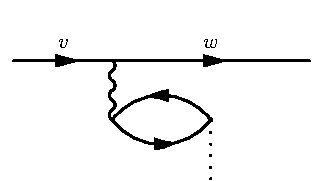
\includegraphics[width=0.195\textwidth]{img/tdhf/meth-CP-direct2}~~~~~
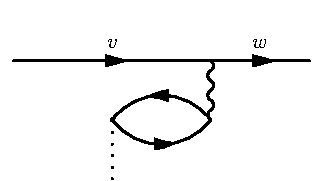
\includegraphics[width=0.195\textwidth]{img/tdhf/meth-CP-direct1}\\
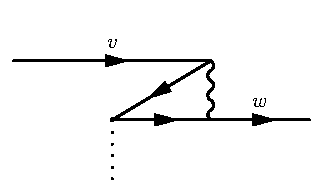
\includegraphics[width=0.195\textwidth]{img/tdhf/meth-CP-exchange1}~~~~~
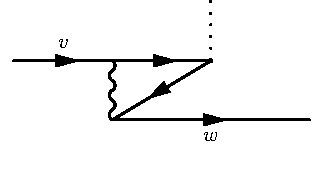
\includegraphics[width=0.195\textwidth]{img/tdhf/meth-CP-exchange2}
\caption{\small Diagrams representing the lowest order direct and exchange core-polarisation (RPA) corrections to the $\bra{w}\hat h\ket{v}$ amplitude.
Wavy line is Columb interaction, dotted line is external field ($\hat h$). All internal lines are summed over: forwards lines are virtual excited states, backward lines are holes in the core.
In higher-order diagrams, each $\hat h$ vertex is corrected again by these four diagrams (RPA).\label{fig:corePol}}
\end{figure}



%Including the core-polarisation, the equation for the corrections becomes:
%\be\label{eq:del-phi-tdhf2}
%\frac{\delta\psi_\vk}{\Upsilon_{\vk,\k}}
% = \frac{\phi_\vk^\infty}{cw}\int_0^r\left\{\phi^0_\vk\|S\right\}\,r^2\d r'
%+ \frac{\phi_\vk^0}{cw}\int_r^\infty\left\{\phi^\infty_\vk\|S\right\}\,r^2\d r'
%\ee
%where
%\begin{multline}
%\left\{\phi_\vk\|S\right\} = 
%-\left\{\phi_\vk\|\hat h\|\psi_\k\right\}
%-\left\{\phi_\vk |V_{\rm nl} |\widetilde{\delta\psi}_\vk\right\}\\
%%
%-\left\{\phi_\vk \|\delta V \|\psi_\k\right\}
%%
%+\delta\en\delta_{\vk\k}\left\{\phi_\vk \|\psi_\k\right\}
%\end{multline}
%[note that the second term on the RHS is just a radial integral, see, e.g., Eq.~(\ref{eq:Vhf-radial})].


%{~\\\color{red}XXX\\
%\textbullet~Use $\delta\psi$, or $\widetilde{\delta\psi}$ in Eq.~(\ref{eq:dV-rme})?? Same after summation over $m$?? Also: Last term??}

%======================================================
\subsubsection{Algebraic method}

%{\em [This is not yet tested or fully implemented in the code]}

The THDF equations  can also be solved using an algebraic method, by expanding the $\chi$ and $\eta$ corrections over a basis of states:
\be
\chi^{\varkappa} = \sum_j a_j x_j \,, \qquad  \eta^{\varkappa} = \sum_j b_j x_j \,, \qquad
\ee
where $\{x_j\}$ is the set of basis orbitals, and $\{a_j/b_j\}$ are the expansion coefficients.
Multiply Eq.~(\ref{eq:tdhf}) from the left by $x_i^\dag$ (and integrate), which yields the matrix equations:
\begin{equation}\begin{split}\label{eq:TDHF-Matrix}
\left[H_{ij} - (\en-\omega)S_{ij}\right] a_j &= -h_{ic} - \delta V_{ic} + \delta\en_{c}S_{ic}\delta_{\kappa_i\k_c} \\
\left[H_{ij} - (\en+\omega)S_{ij}\right] b_j &= -h_{ic}^\dagger - \delta V_{ic}^\dagger + \delta\en_{c}S_{ic}\delta_{\kappa_i\k_c}.
\end{split}\end{equation}
Here,
\begin{equation}\begin{split}
H_{ij} &= \bra{x_i}\hat H_{\rm HF}\ket{x_j} \, , \qquad S_{ij} = \braket{x_i|x_j}\,,  \\
h_{ic} &= \bra{x_i}|\hat h |\ket{\psi_c} \,,\qquad \delta\en_c = \bra{\psi_c}|\hat h + \delta V|\ket{\psi_c}, %+ \delta V?
\end{split}\end{equation}
$\delta V_{ic} $ is given by Eq.~(\ref{eq:dV-rme}), and the delta function means the $\delta\en$ term only appears for partial-wave corrections with $\kappa = \kappa_c$.

There are two ways to proceed.
The simplest way is to solve (\ref{eq:TDHF-Matrix}), which is a pair of linear matrix equations, for the set of expansion coefficients, $a_j$ and $b_j$.
This must be solved for each partial wave correction ($\varkappa_i$) to each core state $c$.
Note, however, that $\delta V$ depends on the corrected states, and thus on $a$ and $b$; so this would have to be solved iteratively.
In another approach, the $\delta V$ term is also expanded in terms of the basis; then no iterations are required, and the equations take the form of a generalised eigenvalue problem, see Ref.~\cite{Johnson1989}.





%======================================================
%\subsection{Core polarisation (RPA diagram technique)}
\subsection[Core polarisation (RPA diagram technique)]{Core polarisation (RPA diagram technique)\footnote{Method implemented in:~/src/MBPT/DiagramRPA.hpp}}

The core polarisation correction to a matrix element can also be taken into account by directly evaluating the four diagrams in Fig.~\ref{fig:corePol}.
To lowest order, the matrix element of operator $\hat h$ is $h_{ij}^{(0)}$. 
The first-order correction is then~\cite{Lindgren1986}:
\begin{align}
\delta h_{ij} &= 
\sum_{ma}\frac{h_{am}^{(0)}\widetilde g_{imja}}{\en_a - \en_m - \omega}
+ \sum_{ma}\frac{h_{ma}^{(0)}\widetilde g_{iajm}}{\en_a - \en_m + \omega},
\label{eq:dh:rpa1}
\end{align}
where
$ \widetilde g_{abcd} =  g_{abcd} -  g_{abdc}$, with 
$g_{abcd}$ being the two-electron Coulomb matrix element (see appendix for definition).
The $a$ sum runs over all occupied core electrons ($n,\k,m$), while $m$ runs over all virtual excited states.

In the RPA method, the lowest-order matrix elements in $\delta h_{ij}$ (\ref{eq:dh:rpa1}) are then replaced with the corrected values. This process is repeated iteratively (for all core states $i$ and $j$) until convergence is reached; i.e., at the $n$th iteration we have:
\begin{multline}
\delta h_{ij}^{n} = \\
\sum_{ma}\Bigg(\frac{(h_{am}^{(0)}+\delta h_{am}^{n-1})\widetilde g_{imja}}{\en_a - \en_m - \omega}
+ \frac{(h_{ma}^{(0)}+\delta h_{ma}^{n-1})\widetilde g_{iajm}}{\en_a - \en_m + \omega}\Bigg).
\end{multline}

The reduced matrix element in the RPA approach is then:
\be
\bra{i}|h|\ket{j}^{\rm RPA} = \bra{i}|h|\ket{j} + \bra{i}|\delta h|\ket{j},
\ee
with
\begin{multline}
\bra{i}|\delta h|\ket{j} = 
\frac{1}{[k]}\sum_{am}(-1)^{j_a-j_i+k}\Bigg(
 \frac{\bra{a}|t|\ket{m}^{\rm RPA}W^k_{imja}}{\en_a-\en_m-\omega}\\
+ (-1)^{j_a-j_m}\frac{\bra{m}|t|\ket{a}^{\rm RPA}W^k_{iajm}}{\en_a-\en_m+\omega}
\Bigg),
\end{multline}
(see appendix for $W^k_{abcd}$ definition; sum is now over {\rm orbitals $n,\k$}).
RPA matrix elements between valence states have the same expression (the equations need only be iterated for the core electrons).
Note that $W$ depends only on the {\em rank} of the operator, so in theory, they need only be calculated once.
In practise, we only calculate $W^k_{imja}$ (e.g.), when $t_{am}\neq0$ -- meaning effectively that $W$ also depends on the operator parity.










%======================================================
\section[Correlation corrections]{Correlation corrections\footnote{Method implemented in:~/src/MBPT/CorrelationPotential.hpp}}

Correlation corrections are the deviation from the pure single-particle picture, and correspond to many-body effects beyond the mean field (Hartree Fock) approximation.
The many-body atomic Hamiltonian may be expressed as
\be
H = \sum_i h_{\rm HF}(\v{r}_i) + \delta V_{\rm corr},
\ee
where $h_{\rm HF}(\v{r}_i)$ is the single-particle HF Hamiltonian (\ref{eq:H-HF}), and
\be\label{eq:residCoul}
\delta V_{\rm corr} = \sum_{i<j}\frac{1}{\v{r}_{ij}} - \sum_iV_{\rm HF}(\v{r}_i)
\ee
is the {\em residual Coulomb interaction} (beyond the mean potential) that may be taken into account perturbatively.
%The perturbative Hamiltonain is
%\be\label{eq:residCoul}
%\delta V_{\rm corr} = \sum_{i<j}\frac{1}{\v{r}_{ij}} - \sum_iV_{\rm HF}(\v{r}_i).
%\ee
We consider the case of an atom with a single valence electron ($v$) above closed shells.
In the single particle picture, this perturbation corresponds to residual interactions of the valence electron with the indevidual electrons in the core.
Starting from the Hartree-Fock method with a $V^{N-1}$ potential, there are no first-order corrections to the wavefunction (that is, corrections involving a single core excitation)~\cite{Lindgren1986}.


{\bf Notation:} In this section (and elsewhere), I use the convention that letters at the beginning of the alphabet {${(a,\,b,\,...)}$} denote occupied core states (or holes),
those from the middle {${(n,\,m,\,...)}$} denote virtual excited states, and
those from the end {${(v,\,w,\,...)}$} denote valence states.
%\footnote{This is the most common convention, e.g.~\cite{JohnsonBook2007}, but is the opposite of that from, e.g.,~\cite{DzubaCPM1988pla}.}.
The letters {${(i,\,j,\,...)}$} are dummy indices that may stand for any state.



%--------------------------------------------------------------------------------------------
\subsection{Second-order correlations: Goldstone technique}

\begin{figure}%[h]
\centering\tiny
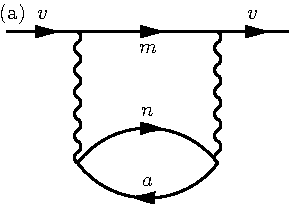
\includegraphics[width=0.185\textwidth]{img/Sigma/Sigma2_a}~~~~~~~
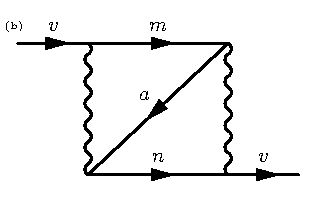
\includegraphics[width=0.185\textwidth]{img/Sigma/Sigma2_b}
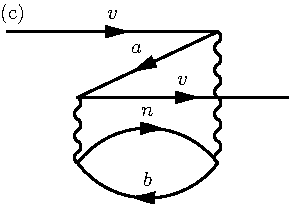
\includegraphics[width=0.185\textwidth]{img/Sigma/Sigma2_c}~~~~~~~
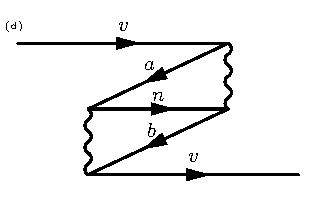
\includegraphics[width=0.185\textwidth]{img/Sigma/Sigma2_d}
\caption{\small Goldstone diagrams for the second-order correlation correction to the energy for valence state $v$. Backward facing lines denote (single-particle) states in the core; $n$ and $m$ are virtual excited states. Diagrams (a) and (c) are direct diagrams, (b) and (d) are corresponding exchange diagrams.\label{fig:Sigma2}}
\end{figure}

This section follows closely the method from Ref.~\cite{DzubaHFS1984}.
Goldstone diagrams for the second-order correction to the valence energy are shown in Fig.~\ref{fig:Sigma2}.
This can be expressed as~\cite{DzubaHFS1984,JohnsonBook2007}:
%\begin{align}\label{eq:dE-SO}
%\delta E_v &= 
%\sum_{amn}
%\frac{g_{vnma}\widetilde g_{vamn}}{\en_v+\en_a - \en_m-\en_n}
%+\sum_{abn}
% \frac{g_{vnab}\widetilde g_{abvn}}{\en_v+\en_n-\en_a-\en_b}  ,
%\end{align}
\begin{align}\label{eq:dE-SO}
\delta E_v &= 
\sum_{amn}
\frac{g_{vamn}\widetilde g_{nmav}}{\en_v+\en_a - \en_m-\en_n}
+\sum_{abn}
 \frac{g_{vnab}\widetilde g_{banv}}{\en_v+\en_n-\en_a-\en_b}  ,
\end{align}
where $m$ and $n$ run over (unoccupied) virtual excited states, and $a$ and $b$ run over (occupied) core states (there is an implicit sum over magnetic quantum numbers here).
The first term corresponds to the diagrams (a) and (b), the second to (c) and (d) [Fig.~\ref{fig:Sigma2}].
Here,
$ \widetilde g_{abcd} =  g_{abcd} -  g_{abdc}$ 
is the anti-symmetrised Coulomb integral (i.e., accounting for exchange), with
\be
 g_{abcd} = \sum_{kq} (-1)^q \bra{a_{\k m}}C^k_{-q}\ket{c_{\k m}} \bra{b_{\k m}}C^k_{q}\ket{d_{\k m}} R^k_{abcd}.
\ee
Summing over magnetic quantum numbers, this gives~\cite{DzubaHFS1984}
\begin{align}
\delta E_v &=\sum_k \frac{1}{[k][j_v]}\Bigg(
 \sum_{amn} \frac{Q^k_{vamn}W^k_{vamn}}{\en_v+\en_a - \en_m-\en_n}
\notag\\&\qquad\qquad\qquad\qquad\qquad
+\sum_{abn}\frac{Q^k_{vnba}W^k_{vnba}}{\en_v+\en_n-\en_b-\en_a} 
 \Bigg),
\end{align}
where we made use of symmetries,  
\begin{align}
Q^k_{abcd} &\equiv (-1)^k \widetilde C^k_{ac}\widetilde C^k_{bd}R^k_{abcd}, \\
W^k_{abcd} &\equiv Q^k_{abcd} + [k] \sum_\lambda \sixj{j_a}{j_c}{k}{j_b}{j_d}{\lambda}Q^\lambda_{abdc} ,
\end{align}
and
$\widetilde C^k_{ab}\equiv  (-1)^{j_a+1/2}  C^k_{ab}$.\footnote{Note: $Q^k$ here differs from that defined in, e.g., Ref.~\cite{DzubaHFS1984} by a factor of $\pm1$; our definition is chosen due to the symmetry properties; see appendix.}
Note that $W$ may be further broken into two terms:
$W^k_{abcd} = Q^k_{abcd} + P^k_{abcd}$, where $Q$ corresponds to the direct term, and $P$ corresponds to exchange.
For the angular reduction, we used the identities (see appendix):
\begin{align}
\sum_{m_{i,j,k,l}}  g_{ijkl} \, g_{lkji}
    &= \sum_\mu \frac{1}{[\mu]} \left( Q^\mu_{ijkl}\right)^2 \\
\sum_{m_{i,j,k,l}}  g_{ijkl} \,g_{klji}
    &=-\sum_\mu \frac{1}{[\mu]}  Q^\mu_{ijkl}P^\mu_{ijkl}.
\end{align}






We define the {\em correlation potential}, $\hat \Sigma$, defined so that its matrix elements correspond to the energy shift: $\bra{v}\Sigma^{(2)}\ket{v} = \delta E_v$.
We define
$Q^{k(\kappa_v)}_{nba}(r)$ (which we will write as $Q^{k(v)}_{nba}$ for brevity, though note it depends only on $\kappa_v$ and not $F_v$), via:
\be
Q^k_{vnba} 
= \braket{F_v|Q^{k(v)}_{nba}}
= \int F_v(r) \, Q^{k(v)}_{nba}(r)\,\d r.
\ee
Note that $Q_{nba}^{k(v)}$ has the form of a radial Dirac spinor [Eq.~(\ref{eq:F-radial})].
% corresponding to angular state $\kappa_v$.
Then, we may express the (energy dependent) second-order correlation potential as
\begin{multline}
\hat \Sigma^{(2)}_{\en} = \\
\sum_{kabnm}\frac{1}{[k][j_v]}\left(
\frac{\ket{Q^{k(v)}_{amn}}\bra{W^{k(v)}_{amn}}}
{\en + \en_a-\en_m-\en_n}
+
\frac{\ket{Q^{k(v)}_{nba}}\bra{W^{k(v)}_{nba}}}
{\en + \en_n-\en_b-\en_a}
\right),
\end{multline}
which is sometimes called the self-energy operator.
This has the form of a sum of Green's functions,
\be
\hat G^{(v)}_{nba}(\en) = \sum_{k}\frac{1}{[k][j_v]}\frac{\ket{Q^{k(v)}_{nba}}\bra{W^{k(v)}_{nba}}}
{\en+\en_n-\en_b-\en_a},
\ee
which can be expressed in (radial) coordinate space as
\be
G^{(v)}_{nba}(r_1,r_2,\en) = \sum_{k}\frac{1}{[k][j_v]}
\frac{Q^{k(v)}_{nba}(r_1)\, W^{k(v)}_{nba}(r_2)}
{\en + \en_n-\en_b-\en_a}.
\ee
Thus the correlation potential may be expressed as
\begin{multline}
\Sigma^{(2)}_{\en}(r_1,r_2) = 
\sum_{abnm}\left[
G^{(v)}_{amn}(r_1,r_2,\en)
+
G^{(v)}_{nba}(r_1,r_2,\en)
\right].
\end{multline}

Note that $G$ is a matrix in (radial) spinor space:
\be
G \propto \matr{f_Q(r_1)f_W(r_2)}{f_Q(r_1)g_W(r_2)}{g_Q(r_1)f_W(r_2)}{g_Q(r_1)g_W(r_2)},
\ee
where $f$ and $g$ are the large and small components of the $Q/W$ radial spinors.
Each of these four terms can themselves be represented as square matrices (on a radial grid).
It is common to only calculate the first ($ff$) term; it is also common to store the $G$ matrix on only a subset of the radial grid.
% (using every 4th grid point, for example, leads to 16x fewer points to calculate/store).
%Note, the inner $y^k_{ab}$ integrals are done using the whole grid!.

%--------------------------------------------------------------------------------------------
\subsection{Correlation potential method (Brueckner orbitals)}


\begin{table*}%[h]
\small
\centering
\caption{\small Removal energies for the lowest $s$, $p$, and $d$ states for the alkali atoms as calculated with the Hartree-Fock and second-order correlation potential methods, and comparison with experiment (Ref.~\cite{NIST}). % ($\Delta = E-E_{\rm Expt.}$).
Note: Calculation of $\Sigma$ used only basis states up to $l=4$; states up to $l=6$ are important, especially for heavy atoms, so these should be taken as an example only.
The inclusion of the correlation potential greatly improves the accuracy of the calculations.\label{tab:alkali-en}}
\begin{tabular}{l D{.}{.}{6.0} l D{.}{.}{5.1} D{.}{.}{2.2} l D{.}{.}{5.1} D{.}{.}{2.3}  |  l D{.}{.}{6.0} l D{.}{.}{5.1} D{.}{.}{3.2} l D{.}{.}{5.1} D{.}{.}{1.2}}
\hline\hline
       & \multicolumn{1}{c}{Expt.}      && \multicolumn{2}{c}{HF}& &\multicolumn{2}{c|}{$\Sigma^{(2)}$ }&           & \multicolumn{1}{c}{Expt.}       && \multicolumn{2}{c}{HF}& &\multicolumn{2}{c}{$\Sigma^{(2)}$ } \\
\cline{4-5} \cline{7-8}  \cline{12-13} \cline{15-16}
\multicolumn{2}{l}{Li $(Z=3)$}          &        &   &      &                &        &  			& \multicolumn{2}{l}{Rb $(Z=37)$}           &          &          &     &&           &          \\
2$s_{1/2}$ & -43487.1 && -43087.3 & -0.9\%   && -43450.6       & -0.08\%  & 5$s_{1/2}$ & -33690.8 && -30570.9 & -9.3\%   && -34162.9       & 1.4\%    \\
2$p_{1/2}$ & -28583.5 && -28232.9 & -1.2\%   && -28539.3       & -0.15\%  & 5$p_{1/2}$ & -21111.9 && -19931.8 & -5.6\%   && -21231.3       & 0.6\%    \\
2$p_{3/2}$ & -28583.1 && -28232.3 & -1.2\%   && -28538.7       & -0.16\%  & 5$p_{3/2}$ & -20874.3 && -19749.6 & -5.4\%   && -20982.4       & 0.5\%    \\
3$d_{3/2}$ & -12204.0 && -12194.4 & -0.08\%  && -12208.3       & 0.04\%   & 4$d_{3/2}$ & -14335.6 && -13112.5 & -8.5\%   && -14415.9       & 0.6\%    \\
3$d_{5/2}$ & -12204.0 && -12194.4 & -0.08\%  && -12208.3       & 0.04\%   & 4$d_{5/2}$ & -14335.2 && -13099.7 & -8.6\%   && -14411.7       & 0.5\%    \\
\hline
\multicolumn{2}{l}{Na $(Z=11)$}          &          &&          &                &&          		& \multicolumn{2}{l}{Cs $(Z=55)$}          &          &          &    &            &          &\\
3$s_{1/2}$ & -41449.5 && -39951.5 & -3.6\%   && -41272.7       & -0.4\%   & 6$s_{1/2}$ & -31406.5 && -27954.1 & -11.0\% & & -32289.8       & 2.8\%    \\
3$p_{1/2}$ & -24493.3 && -24030.4 & -1.9\%   && -24427.8       & -0.3\%   & 6$p_{1/2}$ & -20228.2 && -18790.5 & -7.1\%   && -20488.3       & 1.3\%    \\
3$p_{3/2}$ & -24476.1 && -24014.1 & -1.9\%   && -24409.6       & -0.3\%   & 6$p_{3/2}$ & -19674.2 && -18388.8 & -6.5\%   && -19894.6       & 1.1\%    \\
3$d_{5/2}$ & -12276.6 && -12217.4 & -0.5\%   && -12267.5       & -0.07\%  & 5$d_{5/2}$ & -16907.2 && -14162.6 & -16.2\%  && -17230.9       & 1.9\%    \\
3$d_{3/2}$ & -12276.6 && -12217.4 & -0.5\%   && -12267.4       & -0.07\%  & 5$d_{3/2}$ & -16809.6 && -14138.5 & -15.9\%  && -17090.5       & 1.7\%    \\
\hline
\multicolumn{2}{l}{K $(Z=19)$}          &          &&          &                &&         		 &\multicolumn{2}{l}{Fr $(Z=87)$}          &          &          &   &             &&          \\
4$s_{1/2}$ & -35009.8 && -32370.4 & -7.5\%   && -35316.2       & 0.9\%    & 7$s_{1/2}$ & -32848.9 && -28767.1 & -12.4\%  && -33944.4       & 3.3\%    \\
4$p_{1/2}$ & -22024.6 && -21006.5 & -4.6\%   && -22097.1       & 0.3\%    & 7$p_{1/2}$ & -20611.5 && -18855.2 & -8.5\%   && -20928.5       & 1.5\%    \\
4$p_{3/2}$ & -21966.9 && -20959.4 & -4.6\%   && -22036.1       & 0.3\%    & 7$p_{3/2}$ & -18924.9 && -17655.3 & -6.7\%   && -19124.5       & 1.1\%    \\
3$d_{5/2}$ & -13475.1 && -12747.0 & -5.4\%   && -13516.3       & 0.3\%    & 6$d_{3/2}$ & -16619.0 && -13924.5 & -16.2\%  && -16872.6       & 1.5\%    \\
3$d_{3/2}$ & -13472.8 && -12744.3 & -5.4\%   && -13514.6       & 0.3\%    & 6$d_{5/2}$ & -16419.2 && -13825.5 & -15.8\%  &&                &         \\
\hline\hline
\end{tabular}
\end{table*}




In the {\em correlation potential method}~\cite{DzubaPNC1984,DzubaPNC1985}, the non-local energy-dependent $\Sigma$ operator is added to the single-particle Hartree Fock equation for the valence states:
\be\label{eq:H-Bru}
(H_{\rm HF} + \hat \Sigma_\en)\psi^{\rm (Br)} = \en^{\rm (Br)}\psi^{\rm (Br)}.
\ee
The resulting orbitals are known as Brueckner orbitals\footnote{Note that the exact definition of ``Brueckner'' orbitals varies slightly depending on the source; we use the definition from \cite{DzubaPNC1984}.}, which include the dominating second-order correlation effects.
This means, for example, the dominant correlation corrections can be included into the calculation of matrix elements simply by using the Brueckner orbitals, e.g., $\bra{a^{\rm HF}}{\hat v}\ket{b^{\rm HF}}\to\bra{a^{\rm Br}}{\hat v}\ket{b^{\rm Br}}$.
We will drop the (Br) superscript from here on unless it is necessary to avoid confusion.
The iterations of the Hartree Fock equation for the valence state actually means that certain classes of diagrams are included to all orders; this is called the {\em chaining} of the self-energy operator.
Calculations using the second-order correlation potential method for energies of the lowest states of the alkali atoms are presented in Table~\ref{tab:alkali-en}.



The $\Sigma$ operator should be evaluated at the Hartree Fock energy of the valence state.
However, in order to maintain the orthogonality of the orbitals, all orbitals of the same angular momentum and parity must see the exact same potential.
Therefore, for each $\kappa$, the correlation potential $\Sigma$ must be evaluated at the same energy.
Typically, this is taken as the Hartree-Fock value of the energy of the lowest valence state $v$ of the given symmetry (since this is typically where the highest accuracy is required, and because the correlation corrections are larger for lower states).
Note also that since $|\en_n|\gg|\en_v|$, the correlation potential depends only weakly on $\en_v$ [see Eq.~(\ref{eq:dE-SO})].


To estimate the effect of higher-order correlations, one may introduce scaling factors for the correlation potential, i.e.,
$\Sigma\to\lambda\Sigma$ in Eq.~(\ref{eq:H-Bru}), which are chosen to reproduce the removal energies for the lowest-lying valence states.
For Cs, $\lambda$\,$\approx$\,$0.82$ for $s$ and $0.86$ $p$ states.
This semi-empirical addition leads to much improved agreement with experiment.
See Table~\ref{tab:E1-Cs-comp} for a summary of calculations of electric dipole ($E1$) matrix elements for Cs, and Table~\ref{tab:Cs-Lifetimes} for calculated lifetimes.

\begin{table}%[h]
\small
\centering
\caption{\small 
Reduced $E1$ matrix elements (absolute values) for transitions between the lowest states for Cs as calculated in different approximations, and comparison with experiment (experimental values taken from Ref.~\cite{TohBeta2019}).
RPA means including core-polarisation, $\Sigma$ means using second-order Brueckner orbitals (including core polarisation), and $\lambda\Sigma$ means Brueckner orbitals calculated using scaled correlation potential.
\label{tab:E1-Cs-comp}}
\begin{tabular}{l  D{.}{.}{1.4} D{.}{.}{1.4} D{.}{.}{1.4} D{.}{.}{1.4} D{.}{.}{1.7}}
\hline
\hline
&\multicolumn{1}{c}{HF}&\multicolumn{1}{c}{RPA}&\multicolumn{1}{c}{$\Sigma^{(2)}$}&\multicolumn{1}{c}{$\lambda\Sigma^{(2)}$}&\multicolumn{1}{c}{Expt.}\\
\hline
$6s-6p_{1/2}$ &5.278&4.975&4.404&4.5047&4.5057(16)\\
$6s-6p_{3/2}$ &7.426&7.014&6.193&6.3399&6.3398(22)\\
$6s-7p_{1/2}$ &0.3717&0.2382&0.2996&0.2750&0.2781(44)\\
$6s-7p_{3/2}$ &0.6947&0.5083&0.6049&0.5694&0.5742(57)\\
$7s-6p_{1/2}$ &4.413&4.450&4.234&4.240&4.249(40)\\
$7s-6p_{3/2}$ &6.671&6.713&6.483&6.475&6.489(50)\\
\hline
\hline
\end{tabular}
\end{table}


\begin{table}%[h]
\small
\centering
\caption{\small 
Calculated lifetimes of the lowest states of Cs in various approximations, and comparison with experiment.
Note that calculated frequencies, not experimental values, are used for the HF, RPA and $\Sigma^{(2)}$; since lifetimes scale as $\w^3$, this is the leading source of error.
Experimental results tabulated in Ref.~\cite{Safronova2016b}, except for $5d_{5/2}$ which is from Ref.~\cite{Pucher2019}.
%`Other' refers to theory (CCSDpT) calculations from Ref.~\cite{Safronova2016b}.
\label{tab:Cs-Lifetimes}}
\begin{tabular}{l  D{.}{.}{3.1} D{.}{.}{3.1} D{.}{.}{3.1} D{.}{.}{3.2} D{,}{}{3.5} D{,}{}{4.4}}
\hline
\hline
&\multicolumn{1}{c}{HF}&\multicolumn{1}{c}{RPA}&\multicolumn{1}{c}{$\Sigma^{(2)}$}&\multicolumn{1}{r}{$\lambda\Sigma^{(2)}$}&\multicolumn{1}{c}{Expt.}&\multicolumn{1}{c}{Other$^\dag$}\\
\hline
$6p_{1/2}$ &46.1	&51.8	&31.0	&34.83	&34,.934(94) & 34,.4(12)\\ % [55] of  Safronova, Physical Review A, 94(1), 012505. 
$6p_{3/2}$ &40.9	&45.9	&27.0	&30.42	&30,.460(38) & 30,.0(7)\\
$5d_{3/2}$ &210.4	&227.1	&1077.2	&966.78	&909,(15)& 966,(34)\\
$5d_{5/2}$ &264.2	&284.0	&1494.6	&1348.3	&1353,(5) & 1351,(52) \\
\hline
\hline
\end{tabular}
$^\dag$~{\footnotesize Theory (CCSDpT) calculations from Ref.~\cite{Safronova2016b}}
\end{table}


%\paragraph{\em Correlations into spline basis:}
One may also include the correlation corrections into a set of basis orbitals by adding the correlation potential to the Hartree Fock Hamiltonian when solving the eigenvalue problem for the set of B-splines; i.e.,
\be
H_{ij} \to \bra{S_i}\hat H_{\rm HF}\ket{S_j}  + \bra{S_i}\hat \Sigma_\en\ket{S_j} 
\ee
in Eq.~(\ref{eq:Hij-splines}).
This leads to an (approximately) complete set of orbitals that include correlation effects.
These orbitals may then be used in calculations requiring a summation of a complete set of orbitals; so this method allows the inclusion of correlation corrections into such calculations in a reasonably simple way.
Note that this apprach will lead to a set of orbitals corresponding to orbitals in the core; however, due to the presence of the $\Sigma$ operator, these orbitals will not be orthogonal to the Hartree Fock core orbitals.
These ``core'' orbitals are required for the completeness of the set, and should be included in such summations. %XXX highly-excited auto-ionisation states??
%In the code, I distinguish between the ``basis'' (which doesn't include correlations and should be used in MBPT calculations), and the ``spectrum'', which includes correlations.

%\paragraph{\em Correlations into TDHF:}
The correlation potential can also be taken into account in the time-dependent Hartree Fock method for the valence state:
\be
\left( H_{HF} +\hat\Sigma_\en -  \en -\w \right)X = -\left(\hat h + \delta V - \delta \en \right)\psi_v.
\ee
This gives a means of including the correlation corrections into the Dalgarno-Lewis (Mixed States/Solving Equations) method.
Note that $\delta V$ here is the usual core polarisation correction; the $\Sigma$ operator should not be included into the self-consistent TDHF equations for the core.









%======================================================
%======================================================
%\clearpage
\section{Relativity beyond Dirac-Coulomb (Breit+QED)}


The Dirac equation as presented in Eq.~(\ref{eq:H-manybody})
accounts for the relativistic motion of the electron in the Coulomb field of the nucleus, however, it treats the Coulomb field classically, and treats the electron-electron Coulomb repulsion non-relativistically (see, e.g., Ref.~\cite{BetheBook}).
For high-accuracy calculations, and particularly for atoms with large $Z$, corrections due to the missing relativistic effects become important ($\sim$\,0.1\,--\,1\%).
The two corrections considered here are the
Breit interaction, which contains the dominating relativistic corrections to the electron-electron Coulomb interaction, and 
the radiative quantum electrodynamics (QED) corrections, which are accounted for via the Ginges-Flambaum radiative potential method.




%======================================================
\subsection[Breit interaction]{Breit interaction\footnote{Implemented in: /src/HF/Breit.hpp}}

%\cite{Derevianko2001}

This section mostly follows Ref.~\cite{JohnsonBook2007}; see also \cite{Johnson1988a,Mann1971,Derevianko2001}.
% Treatment of Breit w/ MBPT
%\cite{Derevianko2000,Derevianko2001,DzubaCs2001}
The Breit Hamiltonian accounts for magnetic interactions between electrons (known as the Gaunt interaction), and retardation effects (see, e.g.,~\cite{BetheBook}).
It leads to a correction to the electron-electron Coulomb term in the many-body Hamiltonian (\ref{eq:H-manybody}):
\be
\sum_{ij}\frac{1}{r_{ij}}
\to
\sum_{ij}\left( \frac{1}{r_{ij}} + \hat h^B_{ij}\right),
\ee
where, in the limit of zero frequency, the two-particle Breit Hamiltonian is
\be
\hat h^B_{ij} = - \frac{\v{\a}_i\cdot\v{\a}_j + (\v{\a}_i\cdot\vhat{n}_{ij})(\v{\a}_j\cdot\vhat{n}_{ij})}{2\, \v{r}_{ij}}.
\ee
Frequency-dependent effects can be neglected in most situations, see, e.g., discussion in Refs.~\cite{BetheBook,JohnsonBook2007}.

Inclusion of the Breit Hamiltonian into the Hartree-Fock equations~\cite{Derevianko2001} leads to a correction to the HF potential (\ref{eq:H-HF}):
\be
\hat V_{\rm HF} \to  \hat V_{\rm HF}  + \hat V_{\rm Br} .
\ee
Inclusion into the Hartree-Fock and TDHF equations allows for the inclusion of Breit effects into the calculations of atomic energies and wavefunctions.
(For the TDHF equations, an extra term now appears: $\delta V\to \delta V_{\rm HF}(\delta\phi)+\delta V_{\rm Br}(\delta\phi)$; currently $\delta V_{\rm Br}$ is not implemented in the code, though it may be important.)
%(Currently in the code, Breit Hamiltonian is included only into $H$ for the TDHF equations, 

After integration over angular coordinates, and summation over magnetic quantum numbers, the (non-local) radial Breit operator can be expressed via
\be
\hat V_{\rm Br} F_a(r) = \sum_b^{\rm core}\sum_k \hat B^k_{ba}F_b(r),
\ee
with
\begin{equation}
\hat B^k_{ba} =   \frac{(C^k_{ba})^2 }{[j_a]}  \left[\hat M^k_{ba} + \hat O^k_{ba} + \hat P^k_{ba}\right]
 +
 \frac{(C^k_{-b,a})^2}{[j_a]} \, \hat N^k_{ba}.
\end{equation}
where
$M,N$ are due to the Gaunt effect, $O,P$ are due to retardation, and
 $C^k_{-b,a} \equiv \bra{-\k_b}|C^k|\ket{\k_a}$ (note that only the selection rules depend on the sign of $\k$).


The two Gaunt functions can be expressed as
\begin{multline}
\hat M^k_{ba} = 
\frac{k+1}{2k+3}\left[b_{ba}^{k+1}(r) + \eta^{k+1}_{ba}g_{ba}^{k+1}(r)\right]
\left(\eta_{ba}^{k+1}\hat\s_x - i\hat\s_y\right)\\
-\frac{k}{2k-1}\left[b_{ba}^{k-1}(r) - \eta^{k}_{ba}g_{ba}^{k-1}(r)\right]
\left(\eta_{ba}^{k+1}\hat\s_x + i\hat\s_y\right)
\end{multline}
%
and
%
\begin{equation}
\hat N^k_{ba}(r) = 
 \frac{(\k_b+\k_a)^2}{k(k+1)} \, g^{k}_{ba}(r) \, \hat\s_x,
\end{equation}
%
and the two retardation functions can be expressed as
%
\begin{multline}
\hat O^k_{ba}(r) = 
\frac{(k+1)^2}{[k](2k+3)}\left[b_{ba}^{k+1}(r) + \eta^{k+1}_{ba}g_{ba}^{k+1}(r)\right]
\left(-\eta_{ba}^{k+1}\hat\s_x + i\hat\s_y\right)\\
+\frac{k^2}{[k](2k-1)}\left[b_{ba}^{k-1}(r) - \eta^{k}_{ba}g_{ba}^{k-1}(r)\right]
\left(\eta_{ba}^{k+1}\hat\s_x + i\hat\s_y\right),
\end{multline}
%
and
%
\begin{multline}
\hat P^k_{ba}(r) = 
\frac{k(k+1)}{2[k]}\Big[ P_1(r)\left(\eta_{ba}^{k+1}\hat\s_x - i\hat\s_y\right)  \\ 
-P_2(r)\left(\eta_{ba}^{k}\hat\s_x + i\hat\s_y\right) \Big]
\end{multline}
%
with
%
\begin{align*}
P_1(r) & = 
\left[
b_{0,ba}^{k-1}(r) - \eta^{k}_{ba}g_{0,ba}^{k-1}(r)
 -b_{0,ba}^{k+1}(r) + \eta^{k}_{ba}g_{0,ba}^{k+1}(r)
\right]\\
P_2(r) & = \left[
b_{\infty,ba}^{k-1}(r) + \eta^{k+1}_{ba}g_{\infty,ba}^{k-1}(r) 
-b_{\infty,ba}^{k+1}(r) - \eta^{k+1}_{ba}g_{\infty,ba}^{k+1}(r)
\right].
\end{align*}
%
In the above, $\hat\s$ are Pauli spin matrices, 
$
\eta^k_{ba} = ({\k_b-\k_a})/{k},
$
\begin{multline}
b^k_{ij}(r) = \int_0^r \frac{x^k}{r^{k+1}}[f_ig_j-g_if_j](x)\,\d x  \\
+ \,  \int_r^\infty \frac{r^k}{x^{k+1}}[f_ig_j-g_if_j](x)\,\d x,
\end{multline}
(with $b_0$/$b_\infty$ being just the first/second term), and
\begin{multline}
g^k_{ij}(r) = \int_0^r \frac{x^k}{r^{k+1}}[f_ig_j+g_if_j](x)\,\d x  \\
+ \,  \int_r^\infty \frac{r^k}{x^{k+1}}[f_ig_j+g_if_j](x)\,\d x.
\end{multline}

%-- take a deep breath --




%\clearpage
%======================================================
\subsection[Radiative QED corrections]{Radiative QED corrections\footnote{Functions defined in:~/src/Physics/RadiativePotential.hpp}}

Radiative QED corrections can be included into the wavefunctions using the radiative potential method developed in Ref.~\cite{FlambaumQED2005}, including the (small) finite nuclear size corrections~\cite{GingesQED2015,Ginges2016}.
In this method, an effective potential, $V_{\rm rad}$,
is added to the Hamiltonian before the equations are solved.
The potential can be written as the sum of the Uehling (vacuum polarisation) and self-energy potentials, see Fig.~\ref{fig:QED}.
The self-energy potential itself is written as the sum of the high- and low-frequency electric contributions, and the magnetic contribution:
\be\label{eq:Vrad}
V_{\rm rad}(\v{r}) = V_{\rm Ueh}(r) + V_{\rm SE}^{h}(r) +  V_{\rm SE}^{l}(r) + V_{\rm SE}^{\rm mag}(\v{r}).
\ee


\begin{figure}%[h]
\centering\tiny
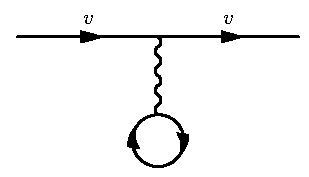
\includegraphics[width=0.185\textwidth]{img/VacuumPol}~~~~~
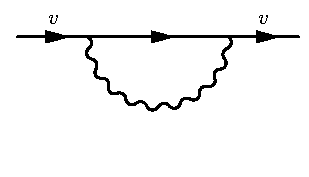
\includegraphics[width=0.185\textwidth]{img/SelfEnergy}
\caption{\small Vacuum polarisation (left) and self-energy (right) diagrams. In the radiative potential method, the self-energy diagram is replaced with an effective local potential~\cite{FlambaumQED2005}.\label{fig:QED}}
\end{figure}

Including this potential into the Hartree-Fock equations (instead of adding it as a subsequent perturbation) gives an important contribution (core relaxation), especially for states with $l>0$.
The first three (electric) terms on the RHS of Eq.~(\ref{eq:Vrad}),
\be
V^{\rm el}(r) =  V_{\rm Ueh}(r) +V_{\rm SE}^{h}(r) + V_{\rm SE}^{l}(r) ,
\ee
are simple scalar terms, and can be included into the calculations simply (e.g., by adding them to the nuclear potential).
The final (magnetic) term, which can be expressed as~\cite{Ginges2016}
\be
V_{\rm SE}^{\rm mag}(\v{r}) = i (\v{\gamma}\cdot\v{n}) H^{\rm mag}(r),
\ee
leads to off-diagonal terms in the Hamiltonian.
Together, they can be included via additions to the radial derivative (\ref{eq:dF}):
\be\label{eq:dF-Hmag}
\p_r F  =\frac{1}{c} \matr 	{c(-{\k}/{r} + H^{\rm mag})} 	{(\en - \hat V + V^{\rm el} + 2c^2)}  {-(\en - \hat V+ V^{\rm el} )} 	 {c({\k}/{r} - H^{\rm mag})}F.
\ee
The sign convention here for $V_{\rm rad}$ (i.e.,\ with $\hat H \to \hat H -V_{\rm rad}$) is from Ref.~\cite{FlambaumQED2005}; in the code I define $H^{\rm el}=-V^{\rm el}$.
%

Detailed expressions for the individual contributions to $V_{\rm rad}$ are given in Refs.~\cite{FlambaumQED2005,GingesQED2015,Ginges2016} -- they involve some rather nasty integrals that must be evaluated carefully.\footnote{Note: there is a small typo in Eq.~(14)  of Ref.~\cite{Ginges2016} $(V^{\rm step}_{\rm high})$; the $r\leq r_N$ and  $r> r_N$ terms should be swapped.}
Due to the presence of double integrals, the high-frequency term $V_{\rm SE}^{hf}$ is quite expensive to calculate.
To speed this up, we calculate it only every $n\approx5$ points along the grid
and use cubic interpolation for the intermediate points.








%======================================================
%\clearpage
%~\\\hrule
\newpage
\appendix

\setcounter{equation}{0}
\setcounter{figure}{0}
\setcounter{table}{0}
\renewcommand{\theequation}{A.\arabic{equation}}
\renewcommand{\thefigure}{A.\arabic{figure}}
\renewcommand{\thetable}{A.\arabic{table}}

\section{Appendix}
\small

Some useful equations and definitions are given here; see also Refs.~\cite{LLVol3,JohnsonBook2007,Sobelman1992,Varshalovich1988,Lindgren1986,Sapirstein1998,DzubaHFS1984}.
Note that notation differs between all these sources, I have introduced some notation not found in the above.

%======================================================
\subsection[Coulomb Integrals]{Coulomb Integrals\label{sec:app-Coulomb}\footnote{Functions to calculate Coulomb integrals defined in:~/src/Coulomb/, and functions for angular coefficients are in:~/src/Angular/}}

The Coulomb integral $g_{abcd}$ can be expressed:
\begin{align}\label{eq:gabcd}
g_{abcd} &\equiv \int\d r_1^3\d r_2^3 \, \psidag_a(\v{r_1})\psidag_b(\v{r_2})\frac{1}{|\v{r}_{12}|}\psi_c(\v{r_1})\psi_d(\v{r_2}) \\
& = \sum_{kq} (-1)^q \bra{\k_a m_a}C^k_{-q}\ket{\k_c m_c} \bra{\k_b m_b}C^k_{q}\ket{\k_d m_d} R^k_{abcd},\notag
\end{align}
where $\v{r}_{12}=|\v{r}_r-\v{r}_2|$ is expanded in terms of spherical tensors (multipolarities, $k$):
\be
\frac{1}{\v{r}_{12}} = \sum_{kq} \frac{r_<^k}{r_>^{k+1}}(-1)^q C^k_{-q}(\v{n}_1)C^k_{q}(\v{n}_2),
\ee
with $r_{<} \equiv \min(r,r')$, and $C^k_{q}$ is a spherical tensor:
\be
C^k_{q} \equiv \sqrt{\frac{4\pi}{2k+1}}Y_{kq}(\v{n}).
\ee
It's also common to define the anti-symmetrised Coulomb integral:
\be
 \widetilde g_{abcd} =  g_{abcd} -  g_{abdc}.
\ee
It is easy to see that $g$ is symmetric under $r_1\leftrightarrow r_2$, and on interchange of initial/final states:
$g_{abcd} = g_{badc} = g_{cdab} = g_{dcba}$.

%
The $R^k_{abcd}$ factor (radial Coulomb integral) is defined:
\begin{align}
R^k_{abcd} =& \int\d r_1 \, \left[f_a(r_1)f_c(r_1) + g_a(r_1)g_c(r_1)\right]\, y^k_{bd}(r_1),
\end{align}
which has symmetries: $c\leftrightarrow a ,~ b\leftrightarrow d  ,~ (ac)\leftrightarrow (bd)$:
\begin{multline}
 R^k_{abcd} =R^k_{cbad} =R^k_{adcb} =R^k_{cdab} \\=R^k_{badc} =R^k_{bcda} =R^k_{dabc} =R^k_{dcba},
\end{multline}
and the symmetric $y^k_{bd}(r) = y^k_{db}(r)$ integral is defined:
\be
y^k_{bd}(r) = \int_0^\infty \frac{r_<^k}{r_>^{k+1}}\left[f_a(r') f_b(r') + g_a(r') g_b(r')\right]\, \d r'.
\ee
The $y^k_{bd}$ are often called Hartree screening functions.

The angular factor is defined:
\begin{align}
C^k_{ab}&\equiv \bra{\k_a}|C^k|\ket{\k_b} ,\\
&= (-1)^{j_a+1/2}\sqrt{[j_a][j_b]}\threej{j_a}{j_b}{k}{-1/2}{1/2}{0}\pi(l_a+l_b+k) \\
&\equiv  (-1)^{j_a+1/2} \widetilde C^k_{ab},
\end{align}
where $\widetilde C^k_{ac}$
 is a short-hand notation that is useful since $\widetilde C^k_{ac} = \widetilde C^k_{ca}$, and $\pi(x)=1$ if $x$ is even, but $=0$ if $x$ is odd.





We further define the useful integrals $Q^k$, $W^k$, and $P^k$:
%\begin{align}
%X^k_{abcd} &\equiv  (-1)^k \bra{\k_a}|C^k|\ket{\k_c} \bra{\k_b}|C^k|\ket{\k_d} R^k_{abcd} \\
% & = (-1)^{j_a+j_b+1}Q^k_{abcd},\notag\\
% Q^k_{abcd} &= (-1)^k \widetilde C^k_{ac}\widetilde C^k_{bd}R^k_{abcd}
%\end{align}
\begin{align}
Q^k_{abcd} &\equiv  (-1)^{k + j_a+j_b+1}\bra{\k_a}|C^k|\ket{\k_c} \bra{\k_b}|C^k|\ket{\k_d} R^k_{abcd} \\
&= (-1)^k \widetilde C^k_{ac}\widetilde C^k_{bd}R^k_{abcd}
\end{align}
and
\begin{align}
W^k_{abcd} &\equiv Q^k_{abcd} + [k] \sum_\lambda \sixj{j_a}{j_c}{k}{j_b}{j_d}{\lambda}Q^\lambda_{abdc} \\
& \equiv Q^k_{abcd}  + P^k_{abcd}
%\\
%Z^k_{abcd} &=  (-1)^{j_a+j_b+1} W^k_{abcd}
\end{align}
$Q^k_{abcd}$  is convenient due to symmetries: $c\leftrightarrow a ,~ b\leftrightarrow d  ,~ (ac)\leftrightarrow (bd)$.% (same as $R$).



%----------------------------------------------------
\subsubsection*{Useful identities}


See also the appendix of Ref.~\cite{DzubaHFS1984} for some very nice general angular identities (though note the minor notational difference between there and here; in particular, the $Q^k$ terms differ by a factor of $\pm1$. My definition is chosen here due to the symmetry properties).

\be
\sum_{m_b}g_{abab} = [j_b] R^0_{abab}.
\ee


%\begin{align}
%\sum_{m_{a,b,n}} \widetilde g_{abvn}g_{vnab} &= \sum_k \frac{1}{[k][j_v]}Z^k_{vnab}X^k_{vnab}\\
%\sum_{m_{b,m,n}} \widetilde g_{vbmn}g_{mnvb} &= \sum_k \frac{1}{[k][j_v]}Z^k_{mnvb}X^k_{mnvb}
%\end{align}


\begin{align}
\sum_{m_{i,j,k,l}}  g_{ijkl} \, g_{lkji}
    &= \sum_\mu \frac{1}{[\mu]} \left( C^\mu_{ik}C^\mu_{jl} R^\mu_{ijkl}\right)^2 \\
    &= \sum_\mu \frac{1}{[\mu]} \left( Q^\mu_{ijkl}\right)^2 
\end{align}

\begin{align}
\sum_{m_{i,j,k,l}}  g_{ijkl} \, g_{klji}
    &=\sum_{\mu \lambda}(-1)^{\mu+\lambda+1}C^\mu_{ik}C^\mu_{jl}C^\lambda_{il}C^\lambda_{jk} \notag \\
    &\phantom{=\sum_{\mu \lambda}}~~\times \sixj{j_i}{j_k}{\mu}{j_j}{j_l}{\lambda}R^\mu_{ijkl}R^\lambda_{ijlk} \\
    &=-\sum_\mu \frac{1}{[\mu]}  Q^\mu_{ijkl}P^\mu_{ijkl}
\end{align}



%=========================================
\subsection{Angular integrals + identities}


%----------------------------------------------------
\subsubsection*{Wigner-Eckhardt theorem}
\begin{multline}
\bra{n_a \k_a m_a}T^k_q\ket{n_b \k_b m_b} \\= (-1)^{j_a-m_a}\threej{j_a}{k}{j_b}{-m_a}{q}{m_b} \bra{n_a \k_a}|T^k|\ket{n_b \k_b}
\end{multline}
\be
\bra{j}|T^k|\ket{j'} = (-1)^{j-j'}\bra{j'}|T^k|\ket{j}^*
\ee
%
\begin{multline}
\bra{J'IF'}|T^k|\ket{JIF} \\= (-1)^{F+J'+I+k}\sqrt{[F'][F]}\sixj{J}{I}{F}{F'}{k}{J'}\bra{J'}|T^k|\ket{J}
\end{multline}
where ($[a]\equiv2a+1$).
%
\be
\sum_{m_a,m_b,q} |\bra{n_a \k_a m_a}T^k_q\ket{n_b \k_b m_b}|^2 = |\bra{n_a \k_a}|T^k|\ket{n_b \k_b}|^2.
\ee







%----------------------------------------------------
\subsubsection*{Clebsch-Gordon coefficients notation}

\begin{align}
\braket{j_1 m_1,j_2m_2|JM} &\equiv (-1)^{j_1-j_2+M}\sqrt{[J]}\threej{j_1}{j_2}{J}{m_1}{m_2}{-M}\\
&\equiv C(j_1,j_2,J; m_1, m_2, M)\\
&\equiv C^{JM}_{j_1m_1,j_2m_2}.
\end{align}
\be
\ket{j_1 j_2;JM} =\sum_{m_1,m_2} \braket{j_1 m_1,j_2m_2|JM} \ket{j_1m_1}\ket{j_2m_2}
\ee






%----------------------------------------------------
\subsubsection*{Some angular integrals + matrix elements}


\be
\sum_{jm}(2j+1)\threej{j_1}{j_2}{j}{m_1}{m_2}{m}\threej{j_1}{j_2}{j}{m_1'}{m_2'}{m} = \delta_{m_1m_1'}\delta_{m_2m_2'}
\ee
\be
\sum_{m_1m_2}(2j+1)\threej{j_1}{j_2}{j}{m_1}{m_2}{m}\threej{j_1}{j_2}{j'}{m_1}{m_2}{m'} = \delta_{jj'}\delta_{mm'}
\ee



\begin{multline}
\int Y_{l'm'}Y_{lm}Y_{LM}\,\d \Omega \\= \sqrt{\frac{[l'][l][L]}{4\pi}}\threej{l'}{l}{L}{0}{0}{0}\threej{l'}{l}{L}{m'}{m}{M}
\end{multline}
\be
\sum_{m_l=-l}^l |Y_{lm_l}|^2 = \frac{2l+1}{4\pi}\quad,\qquad \sum_m |\Omega_{\k m}|^2 = \frac{2j+1}{4\pi}
\ee


%\begin{multline}
%\bra{\k_a}|C^k|\ket{\k_b} \\= (-1)^{j_a+1/2}\sqrt{[j_a][j_b]}\threej{j_a}{j_b}{k}{-1/2}{1/2}{0}\pi(l_a+l_b+k) 
%\end{multline}

\be
\bra{l_a}|C^k|\ket{l_b} = (-1)^{l_a}\sqrt{[l_a][l_b]}\threej{l_a}{l_b}{k}{0}{0}{0}
\ee
%
\be
\bra{n\k}|r_z|\ket{n'\k'} = ({n\k}|r|{n'\k'})\bra{\k}|C^1|\ket{\k'}
\ee



From Ch.~13 of Ref.~\cite{Varshalovich1988}:
\begin{multline}
\bra{jls}|l|\ket{j'l's'} \\= \delta_{ll'}\delta_{ss'}(-1)^{j'+l+s+1}\sqrt{[j][j'][l]l(l+1)}\sixj{j}{1}{j'}{l}{s}{l}
\end{multline}
%
\begin{multline}
\bra{jls}|s|\ket{j'l's'} \\= \delta_{ll'}\delta_{ss'}(-1)^{j+l+s+1}\sqrt{[j][j'][s]s(s+1)}\sixj{j}{1}{j'}{s}{l}{s}
\end{multline}





%======================================================
\subsection{Useful definitions/identities}

\subsubsection*{Dirac matrices}\label{sec:DiracMatrix}

Dirac matrices are defined by the relation:
\be
\{\g^\mu,\g^\nu\} = 2g^{\mu\nu}.
\ee
%and have the properties:
%\be\g^i\g^0 = -\g^0\g^i.\ee
In the Dirac basis, they have the form:
\begin{multline}
\g^0 = \matr{1}{0}{0}{-1} \, , ~~
\g^a = \matr{0}{\s^a}{-\s^a}{0} \, , ~~
\g^5 = \matr{0}{1}{1}{0}.
\end{multline}
It is often convenient to also define:
$\g^5 \equiv i\g^0\g^1\g^2\g^2$.

\subsubsection*{Pauli spin matrices}
\be
\s_x = \matr{0}{1}{1}{0} \, , ~~
\s_y = \matr{0}{-i}{i}{0} \, , ~~
\s_z = \matr{1}{0}{0}{-1}
\ee
\be
\s_i\s_j = i\epsilon_{ijk}\s_k + \delta_{ij} \, , \qquad
[\s_i,\s_j] = 2i\epsilon_{ijk}\s_k
\ee
\be
(\v{\s}\cdot\v{a})\,(\v{\s}\cdot\v{b}) = \v{a}\cdot\v{b} + i\v{\s}\cdot(\v{a}\times\v{b})
\ee
\begin{align}
(\v{\s}\cdot\v{p}) y(r)\Omega_{\k m} &= i\left(y' + \frac{\k+1}{r}y\right)\Omega_{-\k, m} \\
(\v{\s}\cdot\v{n}) \Omega_{\k m} &= -\Omega_{-\k, m},
\end{align}
%\be
%[\v{p},y]\phi = \phi \, (\v{p}y).
%\ee

\subsubsection*{Dirac orbitals (spherical potential, Dirac basis)}
\be
\phi_{n\k m}(\v{r}) = \twocomp
{f_{n\k}(r)\,\Omega_{\k m}(\v{n})}
{ig_{n\k}(r)\,\Omega_{-\k ,m}(\v{n})},
\ee
\begin{align}
\Omega_{\k m}(\v{n}) &=\sum_{\s=\pm1/2} \braket{l,m-\s ,\,1/2,\s|j,m}\,Y_{l,m-\s}(\v{n})\,\chi_{\s} \\
&=
\twocomp
{(-1)^{j-l-1/2}\sqrt{\frac{\k+1/2-m}{2\k+1}}Y_{l,m-1/2}(\theta,\phi)}
{\phantom{(-1)^{j-l-1/2}}\sqrt{\frac{\k+1/2+m}{2\k+1}}Y_{l,m+1/2}(\theta,\phi)}
\end{align}
(with $l \equiv \abs{\k+1/2}-1/2$), where
\be
\k = (l-j)(2j+1) \, ,  ~~
l = \abs{\k+1/2}-1/2\, ,  ~~
j = \abs{\k}-1/2.
\ee
%The DE can be written in radial form as
%\be
% \matr {V - \en} 	{c(-\p_r + \frac{\k}{r})\\}
%	  {c(\p_r + \frac{\k}{r})}	{V-\en-2c^2}
% F_{n\k}=0,
%%\twocomp{f_{n\k}\\}{g_{n\k}} = 0,
%\ee
%%Equation (\ref{eq:Dirac-radial}) 
%which is often written in the equivalent form:
%\be
%\begin{split}\label{eq:Dirac-radial-pair}
%\left(\hat V-\en\right)f - c\left(g' - \frac{\k}{r}g\right) &= 0,\\
%\left(\hat V-2c^2-\en\right)g + c\left(f' + \frac{\k}{r}f\right) &= 0.
%\end{split}
%\ee







%======================================================
~\\\hrule
{\footnotesize
\itemsep0.25em
\bibliography{library}
}
\end{document}
